% !TeX program = latexmk
% !TeX options = -xelatex -synctex=1 -interaction=nonstopmode -file-line-error -outdir=build "%DOC%"
% =============================================================================
% 数学建模竞赛论文通用 LaTeX 模板（完整版）
% -----------------------------------------------------------------------------
% 适用：高教社杯国赛 / 华数杯 / MathorCup / 电工杯 / 深圳杯 / 亚太赛 等
% 编译：xelatex（推荐）或 latexmk -xelatex
% 字库：fontset=fandol（CTeX 自带，无需额外字体文件）
% -----------------------------------------------------------------------------
% 使用说明：
%   1. 全局搜索 【替换】 字样，按提示替换为你的内容
%   2. 摘要采用"六段法"：背景+总方法 / Q1 / Q2 / Q3 / Q4 / 总结，每段必须含具体数值结果
%   3. 图题在下、表题在上；表格一律三线表（无竖线）
%   4. 2026 国赛新规：AI 使用声明置于参考文献之前
%   5. 六大题型（优化/预测/评价/分类/统计/机理）通用，配套规范见 ../01_通用写作规范/00_总索引.md
% =============================================================================

\documentclass[12pt,a4paper,fontset=fandol]{ctexart}

% ============================ 1. 宏包加载 ====================================
\usepackage{geometry}
\geometry{left=2.5cm, right=2.5cm, top=2.5cm, bottom=2.5cm}

\usepackage{amsmath, amssymb}        % 数学公式与符号
\usepackage{amsthm}                  % 定理环境（可选）
\usepackage{booktabs}                % 严格三线表
\usepackage{multirow}                % 跨行表格
\usepackage{array}                   % 表格列格式扩展
\usepackage{makecell}                % 单元格内换行
\usepackage{graphicx}                % 插入图片
\usepackage{float}                   % 强制图表位置 [H]
\usepackage{fancyhdr}                % 自定义页眉页脚
\usepackage{indentfirst}             % 每段首行缩进
\usepackage{caption}                 % 图表标题排版
\usepackage{subcaption}              % 子图排版
\usepackage{longtable}               % 附录长表格跨页
\usepackage{listings}                % 代码高亮
\usepackage{xcolor}                  % 颜色支持
\usepackage{enumitem}                % 列表间距控制
\usepackage{hyperref}                % 超链接与目录（最后加载）
\usepackage{cleveref}                % 智能交叉引用 \cref

% TikZ 流程图（按需启用，编译较慢可注释掉）
\usepackage{tikz}
\usetikzlibrary{shapes.geometric, arrows.meta, positioning, calc, fit, backgrounds}

% ============================ 2. 字体设置 ====================================
\usepackage{newtxtext}               % 正文英文 Times 风格
\usepackage{newtxmath}               % 数学公式 Times 风格
% 中文：ctexart 默认宋体；如需修改：
% \setCJKmainfont{SimSun}[BoldFont=SimHei, ItalicFont=KaiTi]

% ============================ 3. 超链接设置 ==================================
\hypersetup{
    colorlinks=true,
    linkcolor=black,                 % 目录/公式引用
    citecolor=black,                 % 文献引用
    urlcolor=blue,                   % URL
    bookmarksopen=true,
    pdftitle={基于光学追迹与分层降维的定日镜场效率计算与优化设计模型},
    pdfauthor={参赛队}
}

% ============================ 4. 代码块设置 ==================================
\lstset{
    language=Python,                 % 按需改为 MATLAB / R / Julia
    basicstyle=\small\ttfamily,
    keywordstyle=\color{blue},
    commentstyle=\color{green!60!black},
    stringstyle=\color{red!70!black},
    numbers=left,
    numberstyle=\tiny\color{gray},
    frame=single,
    breaklines=true,                 % 自动换行防溢出
    tabsize=4,
    showstringspaces=false,
    literate={_}{{\_}}1,             % 【核心修复】：下划线报错
    captionpos=b                     % 代码标题在下方
}

% ============================ 5. 章节标题格式 ================================
\ctexset{
    section/name={,},
    section/number=\chinese{section}、,           % 一、二、三、
    section/format=\large\bfseries\centering,      % 一级居中加粗
    subsection/number=\arabic{subsection},         % 1 2 3
    subsection/format=\bfseries,                   % 二级加粗
    subsubsection/number=\arabic{subsection}.\arabic{subsubsection},
    subsubsection/format=\itshape                  % 三级斜体
}

% ============================ 6. 正文排版间距 ================================
\renewcommand{\baselinestretch}{1.5}   % 1.5 倍行距
\setlength{\parskip}{0.5em}            % 段间距
\setlength{\parindent}{2em}            % 首行缩进 2 字符

% 图表标题居中
\captionsetup{justification=centering}
\captionsetup[table]{position=above}   % 表题在上
\captionsetup[figure]{position=below}  % 图题在下

% 列表紧凑化
\setlist{nosep, leftmargin=2em}

% ============================ 7. 页眉页脚 ====================================
\pagestyle{fancy}
\fancyhf{}                              % 清空默认
\fancyfoot[C]{\thepage}                 % 页脚居中显示页码
\renewcommand{\headrulewidth}{0pt}      % 不画页眉横线

% ============================ 8. 自定义命令 ==================================
% 摘要页命令：\abstractpage{标题}{摘要正文}
\newcommand{\abstractpage}[2]{%
    \thispagestyle{plain}%
    \pagenumbering{arabic}%
    \setcounter{page}{1}%
    \begin{center}
        {\bfseries\zihao{3} #1}%
    \end{center}
    \vspace{0.5em}
    \begin{center}
        {\bfseries\zihao{4} 摘\quad 要}%
    \end{center}
    \vspace{0.5em}
    #2%
    \vspace{1em}
    \par\noindent\textbf{关键词}：定日镜场；光学效率；射线追迹；分层降维；差分进化
    \newpage
}

% 结果数字加粗便捷命令
\newcommand{\res}[1]{\textbf{#1}}

% ============================ 9. 定理环境（可选）=============================
\newtheorem{definition}{定义}[section]
\newtheorem{theorem}{定理}[section]
\newtheorem{lemma}{引理}[section]

% =============================================================================
\begin{document}

% ============================ 摘要页（六段法）=================================
% 六段式结构：第1段背景+总方法 / 第2段Q1 / 第3段Q2 / 第4段Q3 / 第5段Q4 / 第6段总结
% 硬性要求：①每段开头"针对..."领起 ②第2-5段每段至少一个加粗数字结果 ③方法名必须出现
% 总字数控制 600-900 字，不超过一页。详见 ../01_通用写作规范/摘要六段法通用规范.md
\abstractpage{基于光学追迹与分层降维的定日镜场效率计算与优化设计模型}%
{%
% ---- 第 1 段：背景 + 总方法 ----
针对定日镜场效率计算中阴影遮挡与截断效率强依赖几何追迹、优化中决策变量高维且评价代价高昂两大难点，本文建立以五分量光学效率机理模型为核心、以分层降维为总体策略的计算与优化框架：问题一逐时刻全镜场追迹精确求解，问题二、三将千维布局优化分解为"晶格降维、贪心选镜与全局搜索"的低维组合。

% ---- 第 2 段：问题一（基础模型）----
针对问题一，将光学效率分解为余弦、阴影遮挡、大气透射、截断与反射五分量：前两者解析计算，阴影遮挡效率用镜面采样网格与射线-矩形求交判定（辅以空间近邻筛选），截断效率用 Sobol 序列在光锥内采样、做射线-圆柱求交。对全部 $60$ 个代表时刻逐时追迹，得年平均光学效率$0.5777$、年平均输出热功率$35.32$ MW、单位镜面面积年平均输出热功率$0.5622$ kW/m$^2$，并通过主光线对准、收敛性与对称性等五类检验。

% ---- 第 3 段：问题二（等尺寸优化设计）----
针对问题二，将"额定功率 $60$ MW 下单位面积功率最大"等价变形为"镜面总面积最小"，构建六角晶格生成、快速效率地图、贪心选镜、差分进化搜索与完整复核的五层框架：外层在塔位、镜面尺寸、安装高度与晶格参数共 $8$ 维空间搜索，内层按单镜年均贡献排序选取最少镜面，复核层以 $60$ 时刻完整追迹验证。优化得塔位$(52.4,\,-118.6)$ m、镜面$5.8\times5.8$ m$^2$、安装高度$2.9$ m、定日镜$3025$面，年平均输出热功率$60.08$ MW、单位面积功率$0.5904$ kW/m$^2$，较问题一提升$5.02\%$。

% ---- 第 4 段：问题三（异尺寸优化设计）----
针对问题三，将逐镜尺寸与安装高度离散为档位，内层以"单位面积贡献"为每面镜独立选择最优档位，镜距按 $\max(w_i,\,w_j)+5$ m 约束执行。得定日镜$3062$面、镜面总面积$100742.5$ m$^2$，年平均输出热功率$60.16$ MW、单位面积功率$0.5972$ kW/m$^2$，较问题二提升$1.15\%$，验证了异尺寸布局的增益。

% ---- 第 5 段：总结（模型特色 + 推广价值）----
模型追迹方法在三个问题中完全一致，分层降维将千维布局优化转化为低维搜索与贪心选镜的组合，可推广至大规模塔式光热电站镜场设计。
}% ============================ 目录（可选，按需启用）=========================
% \tableofcontents
% \newpage

% ============================ 一、问题重述 ===================================
\section{问题重述}

定日镜场是一种利用大规模定日镜将太阳辐射聚集至集热器以产生高温热能的太阳能热发电系统。本题要求对给定布局的定日镜场进行光学效率与输出热功率的计算，并进一步对镜场布局进行优化设计。

\textbf{已知条件}包括：
\begin{enumerate}
    \item 镜场位于东经 $98.5^{\circ}$、北纬 $39.4^{\circ}$，海拔 $3000\;\mathrm{m}$ 的圆形区域，半径 $350\;\mathrm{m}$；
    \item 吸收塔建于镜场中心 $(0,\,0)$，集热器为圆柱形外表受光式，中心高度 $80\;\mathrm{m}$，直径 $7\;\mathrm{m}$（半径 $R=3.5\;\mathrm{m}$），高度区间 $[76,\,84]\;\mathrm{m}$；
    \item 吸收塔周围 $100\;\mathrm{m}$ 范围内不安装定日镜；
    \item 定日镜为平面矩形，上下两边始终平行于地面，镜面反射率 $\eta_{\mathrm{ref}} = 0.92$；
    \item 相邻定日镜底座中心最小间距为镜面宽度 $+ 5\;\mathrm{m}$；
    \item 太阳位置按当地时间每月 21 日的 $9{:}00$、$10{:}30$、$12{:}00$、$13{:}30$、$15{:}00$ 五个时刻计算，共 $60$ 个代表时刻。
\end{enumerate}

\textbf{核心任务}是建立定日镜场光学效率的数学模型，分别求解以下三个递进问题：
\begin{itemize}
    \item \textbf{问题一}：给定定日镜尺寸 $6\;\mathrm{m} \times 6\;\mathrm{m}$、安装高度 $4\;\mathrm{m}$，以及附件提供的 $1745$ 面定日镜坐标，计算年平均光学效率、年平均输出热功率及单位镜面面积年平均输出热功率；
    \item \textbf{问题二}：在额定年平均输出热功率 $60\;\mathrm{MW}$ 的约束下，以单位镜面面积年平均输出热功率最大为目标，优化吸收塔位置、定日镜统一尺寸、安装高度及镜面布局；
    \item \textbf{问题三}：在额定功率 $60\;\mathrm{MW}$ 的约束下，允许每面定日镜的尺寸与安装高度不同，进一步优化镜场设计。
\end{itemize}

% ============================ 二、问题分析 ===================================
\section{问题分析}

\subsection{问题一分析}

问题一要求在给定镜场布局下计算光学效率与输出热功率。根据题目定义，单面定日镜的光学效率由五个分量相乘得到：
\begin{equation}
    \eta = \eta_{\mathrm{sb}} \cdot \eta_{\mathrm{cos}} \cdot \eta_{\mathrm{at}} \cdot \eta_{\mathrm{trunc}} \cdot \eta_{\mathrm{ref}}
    \label{eq:eta_decomp}
\end{equation}
其中 $\eta_{\mathrm{sb}}$ 为阴影遮挡效率、$\eta_{\mathrm{cos}}$ 为余弦效率、$\eta_{\mathrm{at}}$ 为大气透射率、$\eta_{\mathrm{trunc}}$ 为截断效率、$\eta_{\mathrm{ref}}$ 为镜面反射率。

\textbf{计算难点}在于阴影遮挡效率与截断效率的几何计算：阴影遮挡效率需要判断镜面之间的几何遮挡关系，涉及射线-矩形求交运算；截断效率需要考虑太阳光锥的发散效应，判断反射光束能否命中集热器圆柱面，涉及射线-圆柱求交运算。余弦效率和大气透射率可由解析公式直接获得。

\textbf{模型选择依据}：鉴于镜场中 $1745$ 面定日镜的阴影遮挡判定需两两比较，直接遍历的计算量为 $O(N^2)$ 级别，本文采用空间近邻筛选策略：对每面镜仅在其预设筛选半径内的候选镜面上进行精确判定，并通过扩大筛选半径的对照实验验证结果的稳定性，从而显著减少耗时较高的射线-矩形求交次数。截断效率的计算采用 Sobol 准随机序列在太阳光锥内采样，该序列具有良好的空间均匀性，且样本数取 $2$ 的幂时便于增量加密。

\subsection{问题二分析}

\textbf{问题特征}：问题二要求在设计额定功率 $60\;\mathrm{MW}$ 的约束下，同时优化吸收塔位置、定日镜统一尺寸、安装高度与全部镜面布局，使单位镜面面积年平均输出热功率最大。直接以全部镜面坐标为连续决策变量时，维数约为 $2N+5$（$N$ 为千量级），且每次评价都需对全部 $60$ 个代表时刻做射线追迹，计算量与不可行解比例均不可接受。

\textbf{模型选择依据}：注意到额定功率固定时，目标"单位面积功率最大"与"镜面总面积最小"等价，镜场设计可以拆解为"布局生成—选镜—评价"三个环节。因此本文采用\textbf{分层降维}策略：外层用差分进化（DE）在塔位、尺寸、安装高度与晶格参数构成的低维空间搜索；内层用六角晶格生成候选镜位，并按单镜贡献贪心选取最少镜面；复核层用与问题一同口径的完整追迹验证。相比直接将全部镜位作为优化变量的做法，该策略将优化维数降低两个量级，且六角晶格天然满足相邻间距约束，具有可行性高、计算量可控的优势。

\subsection{问题三分析}

\textbf{问题特征}：问题三进一步允许每面定日镜的尺寸与安装高度各不相同，决策变量维数由问题二的 $2N+5$ 扩展至约 $5N$，且镜面尺寸差异使相邻间距约束（与镜宽耦合）与非均匀布局下的阴影遮挡关系更加复杂，直接搜索几乎不可行。

\textbf{模型选择依据}：针对本问题的大规模维度与搜索空间的双重复杂性，本文在问题二的分层框架上扩展：外层仍搜索塔位与晶格全局参数，内层将镜面尺寸与安装高度离散为有限档位，对每面候选镜独立选择"单位面积贡献"最优的档位，并按贡献贪心选镜。该策略把"逐镜连续尺寸"的高维问题降为"档位离散选择"，在保持与问题一、二同一追迹口径的同时控制了搜索规模。

\subsection{研究技术路线}

本文的研究技术路线为：首先建立统一的太阳几何与五分量光学效率计算模型，按 $60$ 个代表时刻逐时追迹，完成问题一的计算与五类模型检验；其次将问题二等价变形为"总面积最小"约束优化，设计"六角晶格布局生成 + 快速效率地图 + 内层贪心选镜 + 外层差分进化 + 完整射线复核"的分层求解框架，得到等尺寸最优设计方案；再次在问题三中引入逐镜尺寸与安装高度的档位离散化，扩展同一框架求解异尺寸设计；最后对三个问题的结果进行约束验证、精度复核与敏感性分析，并按模板导出结果文件。整体研究思路如图~\ref{fig:framework} 所示。

\begin{figure}[H]
    \centering
    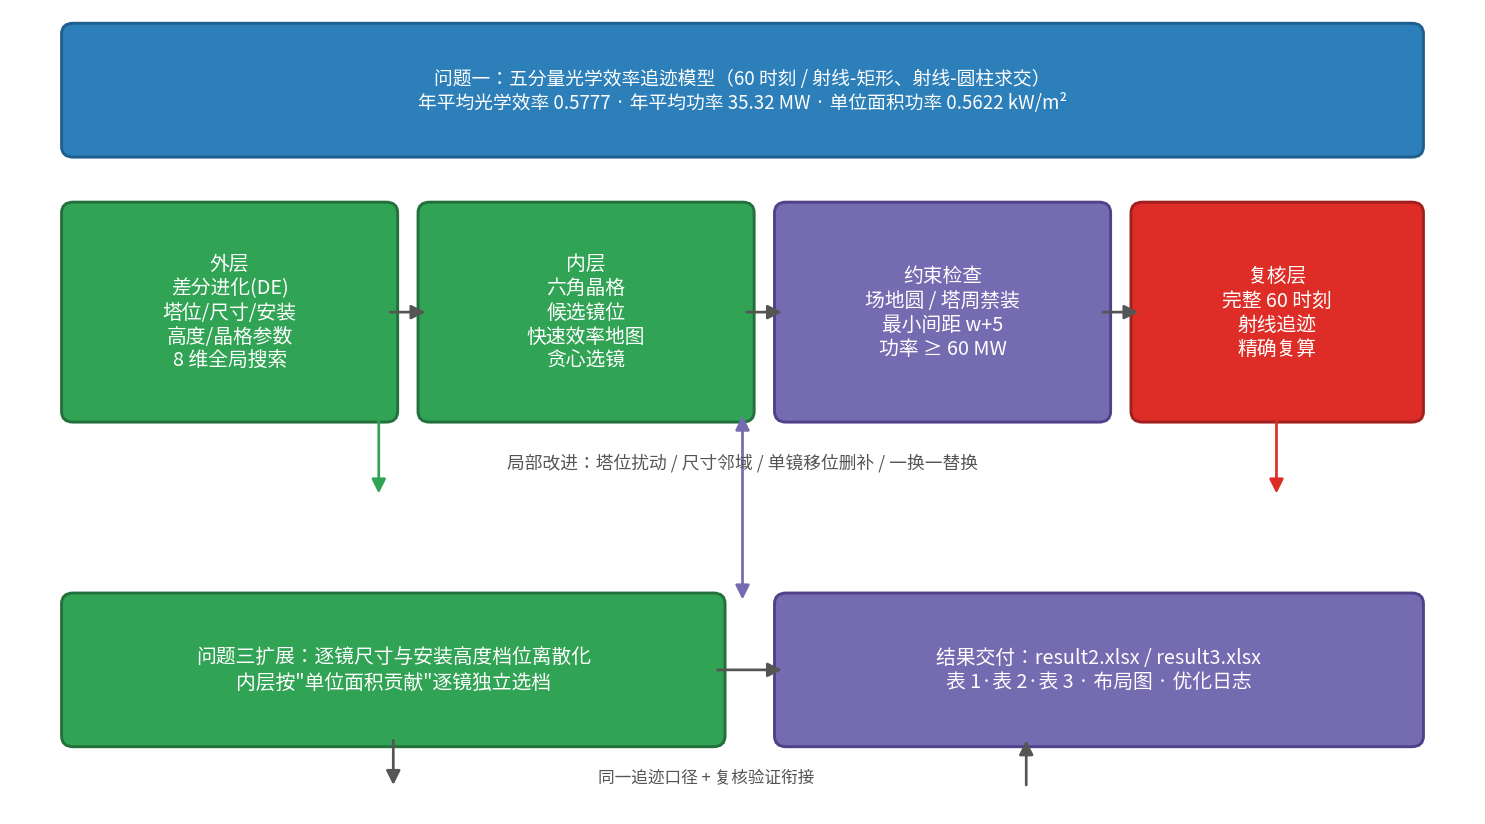
\includegraphics[width=0.95\textwidth]{figures/fig1_framework.png}
    \caption{研究技术路线流程图}
    \label{fig:framework}
    \begin{center}
        \footnotesize 三层求解框架：问题一建立追迹口径基准；问题二在低维空间搜索+贪心选镜；问题三扩展逐镜尺寸档位；各层之间以同一五分量模型与复核验证衔接。
    \end{center}
\end{figure}

% ============================ 三、模型假设 ===================================
\section{模型假设}

为了简化模型并聚焦于核心问题，我们做出以下合理假设：
\begin{enumerate}
    \item 假设吸收塔为与集热器等半径的圆柱（保守近似，题目未给出塔身半径），两者合并为 $z \in [0,\,84]\;\mathrm{m}$ 的连续圆柱体；塔身圆柱仅用于塔影遮挡判定，集热器接收判定仍只取 $z \in [76,\,84]\;\mathrm{m}$。敏感性检验表明，塔身半径在 $2$--$4\;\mathrm{m}$ 范围内变化时，最不利时刻（冬季低太阳角）受塔影遮挡的采样点占比仅 $0.24\%$--$0.56\%$，相对 $3.5\;\mathrm{m}$ 基准的变化不超过 $0.2$ 个百分点，该假设对结果的影响可忽略；
    \item 假设定日镜为理想平面镜，不考虑镜面弯曲变形；
    \item 假设忽略定日镜跟踪误差及风载引起的镜面偏转，镜面法向量精确指向目标点；
    \item 假设太阳视圆盘半角取 $\sigma = 4.65\;\mathrm{mrad}$，将太阳光束视为半角为 $\sigma$ 的锥形光束，且视圆盘内辐射能流密度均匀分布，不考虑临边昏暗、跟踪误差及镜面面形误差；
    \item 假设月均性能取每月 21 日五个时刻的等权平均，年均性能取 12 个月的等权平均；
    \item 假设按晴天大气模型计算法向直射辐照度（DNI），不考虑云量、气溶胶等天气因素；
    \item 假设忽略镜面间多次反射与地面反射对能量传递的影响；
    \item 假设题目给定的当地时间即为当地太阳时，不额外进行经度时差修正。
\end{enumerate}

% ============================ 四、符号说明 ===================================
\section{符号说明}

\renewcommand{\arraystretch}{1.15}
\small
\begin{longtable}{p{0.16\textwidth}p{0.36\textwidth}p{0.16\textwidth}}
    \toprule
    符号 & 意义说明 & 单位 \\
    \midrule
    \endfirsthead
    \toprule
    符号 & 意义说明 & 单位 \\
    \midrule
    \endhead
    \midrule
    \multicolumn{3}{r}{\small 接下页} \\
    \endfoot
    \bottomrule
    \endlastfoot
    $H_i, \mathbf{n}_i$ & 镜心坐标、法向量 & m, — \\
    $\mathbf{s}, \mathbf{r}_i$ & 太阳方向、反射方向单位向量 & — \\
    $\varphi, \delta, \omega$ & 地理纬度、赤纬角、太阳时角 & rad \\
    $\alpha_s, D$ & 太阳高度角、相对春分天数 & rad, 天 \\
    $G_0$ & 太阳常数（$1.366$） & kW/m$^{2}$ \\
    $\eta_{\mathrm{cos}}, \eta_{\mathrm{sb}}, \eta_{\mathrm{at}}$ & 余弦、阴影遮挡、大气透射效率 & — \\
    $\eta_{\mathrm{trunc}}, \eta_{\mathrm{ref}}, \eta$ & 截断、反射、综合效率 & — \\
    $W, h$ & 镜面边长（问题一 $W=6$）、安装高度（问题一 $h=4$） & m \\
    $R, A_i, N$ & 集热器半径（$R=3.5$）、镜面面积、镜面总数（$N=1745$） & m, m$^{2}$, 面 \\
    $\sigma, d_{\mathrm{HR}}, R_c$ & 光锥半角（$\sigma=4.65$）、镜-塔距离、遮挡筛选半径 & mrad, m, m \\
    DNI, $P, q$ & 法向直射辐照度、镜场输出热功率、单位镜面面积输出热功率 & kW/m$^{2}$, MW, kW/m$^{2}$ \\
    $P_{\mathrm{rated}}, T$ & 额定输出热功率（$60$）、塔位坐标 $T=(x_T,y_T)$ & MW, m \\
    $w, H, a$ & 镜面宽度、高度、安装高度（问题二、三优化变量） & m \\
    $A_{\mathrm{total}}, \Phi_i, d, \theta$ & 镜面总面积、年均能量贡献、晶格间距、旋转角 & m$^{2}$, kW, m, rad \\
    $s_{\mathrm{shadow},i}, \lambda$ & 年均阴影遮挡系数、罚函数系数 & ---
\end{longtable}

% ============================ 五、模型的建立与求解 ===========================
\section{模型的建立与求解}

定日镜场效率计算与优化设计遵循"先建立机理模型、再分层求解优化"的数学建模思路\cite{1}，问题一建立与题目口径一致的五分量效率基准模型，问题二、三在此基础上分层降维求解优化设计。

\subsection{问题一：光学效率计算模型}

问题一要求在给定镜场布局下计算年平均光学效率与输出热功率。根据题目定义，单面定日镜的光学效率由五个分量相乘得到：
\begin{equation}
    \eta = \eta_{\mathrm{sb}} \cdot \eta_{\mathrm{cos}} \cdot \eta_{\mathrm{at}} \cdot \eta_{\mathrm{trunc}} \cdot \eta_{\mathrm{ref}}
    \label{eq:eta_total}
\end{equation}
其中 $\eta_{\mathrm{sb}}$ 为阴影遮挡效率、$\eta_{\mathrm{cos}}$ 为余弦效率、$\eta_{\mathrm{at}}$ 为大气透射率、$\eta_{\mathrm{trunc}}$ 为截断效率、$\eta_{\mathrm{ref}} = 0.92$ 为镜面反射率（题目附录建议值）。

求解流程分为五步：首先由日期与时刻计算太阳赤纬角、时角与太阳方向向量；其次由反射定律确定每面镜的法向量，解析计算余弦效率与大气透射率；再次在每面镜面上布设采样网格，通过射线-矩形求交判定塔影、镜间阴影与挡光，得到阴影遮挡效率；然后用 Sobol 序列在太阳光锥内采样，通过射线-圆柱求交判定命中率，得到截断效率；最后将五个分量相乘得到综合光学效率，并按 $60$ 个代表时刻汇总为月均与年均指标。下面依次建立各分量的计算模型。

\subsubsection{数据预处理}

附件给出了 $1745$ 面定日镜中心的水平坐标。建模前先对数据进行质量检查：镜面总数恰为 $1745$ 面，无缺失、无重复坐标；镜心到吸收塔的水平距离最小 $107.9\;\mathrm{m}$、最大 $337.1\;\mathrm{m}$，全部落在题目规定的 $[100,\,350]\;\mathrm{m}$ 环形安装区域内；相邻镜心的最小间距为 $11.68\;\mathrm{m}$，满足"相邻定日镜底座中心间距比镜面宽度多 $5\;\mathrm{m}$ 以上"（$6+5=11\;\mathrm{m}$）的约束。数据质量满足建模要求，镜场总面积 $A_{\mathrm{total}} = 1745 \times 36 = 62820\;\mathrm{m}^{2}$。

\subsubsection{太阳几何模型}

太阳位置是光学效率计算的基础\cite{5}。需要确定三个几何量：太阳赤纬角 $\delta$、太阳时角 $\omega$ 和太阳方向单位向量 $\mathbf{s}$。

\textbf{（1）太阳赤纬角}

太阳赤纬角 $\delta$ 由日期决定，表示太阳直射点相对于赤道的偏角。以春分（3 月 21 日）为第 $0$ 天，$D$ 为给定日期相对春分的天数，则：
\begin{equation}
    \sin\delta = \sin\!\left(\frac{2\pi D}{365}\right) \cdot \sin(23.45^{\circ})
    \label{eq:declination}
\end{equation}
每月 21 日对应的天数 $D$ 如表~\ref{tab:month_D} 所示。

\begin{table}[H]
    \centering
    \caption{每月 21 日相对春分的天数 $D$}
    \label{tab:month_D}
    \small
    \begin{tabular}{ccccccccccccc}
        \toprule
        月份 & 1 & 2 & 3 & 4 & 5 & 6 & 7 & 8 & 9 & 10 & 11 & 12 \\
        \midrule
        $D$ & 306 & 337 & 0 & 31 & 61 & 92 & 122 & 153 & 184 & 214 & 245 & 275 \\
        \bottomrule
    \end{tabular}
\end{table}

\textbf{（2）太阳时角}

太阳时角 $\omega$ 表征一天中太阳的东升西落，当地时间 $ST$（单位：h）与时角的关系为：
\begin{equation}
    \omega = \frac{\pi}{12}(ST - 12)
    \label{eq:hour_angle}
\end{equation}
正午 $ST=12$ 时 $\omega=0$，上午 $\omega<0$，下午 $\omega>0$。本题取每月 21 日的 $9{:}00$、$10{:}30$、$12{:}00$、$13{:}30$、$15{:}00$ 五个代表时刻。

\textbf{（3）太阳高度角与方向向量}

太阳高度角 $\alpha_s$ 满足：
\begin{equation}
    \sin\alpha_s = \cos\delta\cos\varphi\cos\omega + \sin\delta\sin\varphi
    \label{eq:altitude}
\end{equation}
其中 $\varphi = 39.4^{\circ}$ 为当地地理纬度。

在镜场坐标系（$x$ 正东、$y$ 正北、$z$ 正上）中，太阳方向单位向量 $\mathbf{s}$ 为：
\begin{equation}
    \mathbf{s} = \frac{1}{|\mathbf{s}_0|}\begin{pmatrix} -\cos\delta\sin\omega \\ \cos\varphi\sin\delta - \sin\varphi\cos\delta\cos\omega \\ \sin\alpha_s \end{pmatrix}
    \label{eq:sun_vector}
\end{equation}
该向量由太阳高度角和方位角经坐标变换直接得到，避免了先求方位角再转笛卡尔坐标时上午/下午信息丢失的问题。

\subsubsection{法向直射辐照度}

法向直射辐照度 DNI（Direct Normal Irradiance）是垂直于太阳光线的单位面积上接收到的太阳辐射功率，按题目附录给出的经验公式计算\cite{3}：
\begin{equation}
    \mathrm{DNI} = G_0\left[a + b\exp\!\left(-\frac{c}{\sin\alpha_s}\right)\right]
    \label{eq:DNI}
\end{equation}
其中 $G_0 = 1.366\;\mathrm{kW/m^2}$ 为太阳常数，$\alpha_s$ 为太阳高度角，系数 $a,b,c$ 与海拔 $H$（单位：km）有关：
\begin{equation}
    \begin{cases}
        a = 0.4237 - 0.00821(6 - H)^2 \\[4pt]
        b = 0.5055 + 0.00595(6.5 - H)^2 \\[4pt]
        c = 0.2711 + 0.01858(2.5 - H)^2
    \end{cases}
    \label{eq:DNI_coeff}
\end{equation}
本镜场海拔 $H = 3\;\mathrm{km}$，代入得 $a = 0.3498$，$b = 0.5784$，$c = 0.2757$。低太阳角时 $\sin\alpha_s$ 趋于 $0$，指数项 $\exp(-c/\sin\alpha_s)$ 趋于 $0$，DNI 趋近 $G_0 \cdot a$；高太阳角时指数项贡献增大，DNI 增大。

\subsubsection{余弦效率}

余弦效率 $\eta_{\mathrm{cos}}$ 反映太阳光线入射角对镜面有效采光面积的衰减。设第 $i$ 面定日镜中心坐标为 $\mathbf{H}_i = (x_i, y_i, h)$，集热器中心坐标为 $\mathbf{C} = (0, 0, 80)\;\mathrm{m}$，则镜心指向集热器中心的单位向量为：
\begin{equation}
    \mathbf{t}_i = \frac{\mathbf{C} - \mathbf{H}_i}{|\mathbf{C} - \mathbf{H}_i|}
    \label{eq:t_vector}
\end{equation}
根据反射定律，定日镜法向量应平分太阳方向 $\mathbf{s}$ 与反射目标方向 $\mathbf{t}_i$ 的夹角：
\begin{equation}
    \mathbf{n}_i = \frac{\mathbf{s} + \mathbf{t}_i}{|\mathbf{s} + \mathbf{t}_i|}
    \label{eq:normal}
\end{equation}
余弦效率定义为太阳方向在法向上的投影：
\begin{equation}
    \eta_{\mathrm{cos},i} = \mathbf{s} \cdot \mathbf{n}_i
    \label{eq:eta_cos}
\end{equation}
当太阳光线垂直入射时 $\eta_{\mathrm{cos}} = 1$（最大），入射角越大余弦效率越低。该值仅依赖镜面位置与太阳方向，与镜间布局无关，可对所有镜面向量化计算。

\subsubsection{大气透射率}

太阳光从镜面反射后到达集热器的过程中，大气衰减与传播距离有关。设镜面中心到集热器中心的距离为 $d_{\mathrm{HR}}$（单位：m），大气透射率按题目附录的经验公式计算\cite{4}：
\begin{equation}
    \eta_{\mathrm{at}} = 0.99321 - 0.0001176\,d_{\mathrm{HR}} + 1.97 \times 10^{-8} \times d_{\mathrm{HR}}^{2}, \quad d_{\mathrm{HR}} \leq 1000\;\mathrm{m}
    \label{eq:eta_at}
\end{equation}
其中距离 $d_{\mathrm{HR}}$ 为：
\begin{equation}
    d_{\mathrm{HR}} = |\mathbf{C} - \mathbf{H}_i| = \sqrt{x_i^2 + y_i^2 + (80 - h)^2}
    \label{eq:d_HR}
\end{equation}
$\eta_{\mathrm{at}}$ 仅依赖镜面位置，不随时刻变化，可一次性预计算。

\subsubsection{阴影遮挡效率}

阴影遮挡效率 $\eta_{\mathrm{sb}}$ 是本模型计算量最大的分量，按张平等\cite{2}给出的分类，需要考虑三层遮挡关系。

\textbf{（1）塔身阴影}

吸收塔（含集热器）简化为半径 $R_t = 3.5\;\mathrm{m}$、高度 $[0, 84]\;\mathrm{m}$ 的圆柱体。镜面上的采样点 $P$ 沿太阳方向 $\mathbf{s}$ 发射射线，若在到达太阳之前先碰到塔身圆柱，则该点被塔阴影遮挡。光线-圆柱求交归结为水平分量的二次方程：
\begin{equation}
    A\lambda^2 + B\lambda + C = 0
    \label{eq:ray_cyl}
\end{equation}
其中 $A = s_x^2 + s_y^2$，$B = 2(P_x s_x + P_y s_y)$，$C = P_x^2 + P_y^2 - R_t^2$。取最小正根 $\lambda$，若交点高度 $P_z + \lambda s_z \in [0, 84]\;\mathrm{m}$，则该点被遮挡。

\textbf{（2）镜间阴影与挡光}

相邻镜面之间的遮挡分为两类：
\begin{itemize}
    \item \textbf{阴影}：采样点沿太阳方向 $\mathbf{s}$ 被前排镜面遮挡（阻挡阳光到达镜面）；
    \item \textbf{挡光}：反射光线沿 $\mathbf{r}_i = 2(\mathbf{s} \cdot \mathbf{n}_i)\mathbf{n}_i - \mathbf{s}$ 方向被前排镜面阻挡（反射光无法到达集热器）。
\end{itemize}
阴影与挡光判定均按太阳中心主光线方向进行：太阳锥角 $\sigma = 4.65\;\mathrm{mrad}$ 很小，在 $20\;\mathrm{m}$ 筛选半径内由光锥造成的半影宽度仅约 $2\sigma \times 20 \approx 0.19\;\mathrm{m}$，远小于镜面边长 $6\;\mathrm{m}$，该小发散角近似合理；光锥的发散效应仅在截断效率计算中考虑。

两者判定方法相同：将遮挡镜面建模为矩形平面，判断采样点发出的射线是否与矩形相交。设第 $j$ 面候选遮挡镜中心为 $\mathbf{H}_j$、法向为 $\mathbf{n}_j$、镜面坐标系基向量为 $\mathbf{u}_j$（宽度方向）、$\mathbf{v}_j$（高度方向），射线方向为 $\mathbf{d}$（$\mathbf{s}$ 或 $\mathbf{r}_i$），求交过程为：
\begin{enumerate}
    \item 射线与镜面 $j$ 所在平面的交点参数：$\lambda = \dfrac{(\mathbf{H}_j - P) \cdot \mathbf{n}_j}{\mathbf{d} \cdot \mathbf{n}_j}$
    \item 交点在镜面 $j$ 坐标系中的局部坐标：$u = (Q - \mathbf{H}_j) \cdot \mathbf{u}_j$，$v = (Q - \mathbf{H}_j) \cdot \mathbf{v}_j$
    \item 判定：若 $\lambda > 0$ 且 $|u| \leq W/2$、$|v| \leq W/2$，则射线被遮挡镜面 $j$ 阻挡
\end{enumerate}
每面镜的遮挡判定只需在空间近邻候选集内进行：太阳高度角最低（$14.4^{\circ}$）时，镜间阴影在相邻镜面高度上的水平延伸约为 $12\;\mathrm{m}$，取筛选半径 $R_c = 20\;\mathrm{m}$ 可覆盖绝大多数遮挡事件。以最不利时刻（12 月 21 日 9:00）为例，$20\;\mathrm{m}$ 筛选与全镜场两两判定的输出热功率偏差仅约 $0.1\%$（残余差异来自镜面边缘采样点的少量远距离遮挡事件），且 $30\;\mathrm{m}$ 及以上筛选半径与全镜场结果完全一致；年均口径下 $20\;\mathrm{m}$ 与 $40\;\mathrm{m}$ 的光学效率相对差仅 $0.004\%$（表~\ref{tab:convergence}），可忽略。该策略使每面镜的平均候选镜数量由 $1745$ 降至约 $6$ 个，大幅减少射线-矩形求交次数。

\textbf{（3）阴影遮挡效率}

每面镜面上布置 $10 \times 10$ 的均匀采样网格（共 $100$ 个采样点），统计未被任何遮挡覆盖的有效采样点比例：
\begin{equation}
    \eta_{\mathrm{sb},i} = \frac{\text{有效采样点数}}{\text{总采样点数}}
    \label{eq:eta_sb}
\end{equation}

\subsubsection{截断效率}

太阳光并非理想平行光，而是半角 $\sigma = 4.65\;\mathrm{mrad}$ 的锥形光束\cite{2}。反射后的光锥可能部分超出集热器接收范围，截断效率 $\eta_{\mathrm{trunc}}$ 度量反射光锥命中集热器的比例。

\textbf{（1）光锥内入射方向采样}

采用 Sobol 准随机序列在光锥内生成 $K$ 条入射方向（$K = 1024$，$2$ 的幂以保证 Sobol 平衡性）。光锥坐标系中，第 $k$ 条光线与主光线（太阳方向 $\mathbf{s}$）的夹角为：
\begin{equation}
    \sigma_k = \sigma_{\max} \cdot \sqrt{u_{1,k}}, \quad \tau_k = 2\pi \cdot u_{2,k}
    \label{eq:cone_sample}
\end{equation}
其中 $(u_{1,k}, u_{2,k})$ 为 Sobol 二维准随机数，$\sqrt{u_1}$ 保证圆盘面积均匀采样。将光锥坐标系下的方向转换回镜场坐标系，得到入射方向 $\mathbf{d}_k$。

\textbf{（2）反射光锥与集热器圆柱求交}

对每条入射方向 $\mathbf{d}_k$，计算反射方向：
\begin{equation}
    \mathbf{r}_k = 2(\mathbf{d}_k \cdot \mathbf{n}_i)\mathbf{n}_i - \mathbf{d}_k
    \label{eq:cone_reflect}
\end{equation}
将反射光线与集热器圆柱（半径 $R = 3.5\;\mathrm{m}$，高度 $[76, 84]\;\mathrm{m}$）按式~\eqref{eq:ray_cyl} 求交，若交点高度落在 $[76, 84]\;\mathrm{m}$ 内，则该光线被集热器接收。

\textbf{（3）截断效率}

截断效率定义为被接收的光线占有效采样点发出的总光线的比例：
\begin{equation}
    \eta_{\mathrm{trunc},i} = \frac{\text{命中集热器的光线数}}{\text{有效采样点数} \times K}
    \label{eq:eta_trunc}
\end{equation}
其中分母以未被阴影遮挡的有效采样点为准，与题目附录中"镜面全反射能量减去阴影遮挡损失能量"的口径一致——阴影遮挡损失已计入 $\eta_{\mathrm{sb}}$，此处不再重复扣除。

从物理机理上看，定日镜为平面镜而非聚焦镜，镜面上不同位置发出的主光线近似平行，反射后在集热器处形成与镜面尺寸相当的光斑。截断损失来自两个相互制约的效应：\textbf{（1）横向溢出}——光斑直径 $W + 2\sigma d_{\mathrm{HR}}$ 随镜塔距离增大而增大，远场镜面（如 $d_{\mathrm{HR}} = 300\;\mathrm{m}$ 时光斑直径约 $8.8\;\mathrm{m}$）超出集热器直径 $7\;\mathrm{m}$，两侧光线无法被接收；\textbf{（2）纵向溢出}——近场镜面的反射光束以陡峭仰角入射集热器，光束在圆柱面上的竖直足迹被拉长（约为 $(W + 2\sigma d_{\mathrm{HR}})/\cos\theta_i$，$\theta_i$ 为反射方向仰角），超出集热器高度 $8\;\mathrm{m}$ 的部分光线从顶部或底部逸出。两者权衡下，截断效率随镜塔距离呈先升后降的非单调关系，如表~\ref{tab:trunc_distance} 所示：$100$--$150\;\mathrm{m}$ 组最低（约 $0.85$），$200$--$300\;\mathrm{m}$ 组最高（约 $0.96$），$300$--$350\;\mathrm{m}$ 组回落至约 $0.95$。该规律在各代表时刻一致，全场平均截断效率约 $0.94$，与上述机理相符。

\begin{table}[H]
    \centering
    \small
    \caption{截断效率随镜塔水平距离的分组统计（6 月 21 日正午）}
    \label{tab:trunc_distance}
    \begin{tabular}{lcc}
        \toprule
        镜塔水平距离 (m) & 镜面数 & 平均截断效率 \\
        \midrule
        100--150 & 268 & 0.8589 \\
        150--200 & 260 & 0.9457 \\
        200--250 & 403 & 0.9683 \\
        250--300 & 439 & 0.9628 \\
        300--350 & 375 & 0.9518 \\
        \bottomrule
    \end{tabular}
\end{table}

\subsubsection{综合光学效率与输出热功率}

综合光学效率由五个分量相乘得到，如式~\eqref{eq:eta_total} 所示。镜场平均光学效率按镜面面积加权：
\begin{equation}
    \bar{\eta} = \frac{\sum_{i=1}^{N} A_i \cdot \eta_i}{\sum_{i=1}^{N} A_i}
    \label{eq:eta_field}
\end{equation}
单面定日镜在时刻 $t$ 的输出热功率为：
\begin{equation}
    E_i(t) = \mathrm{DNI}(t) \cdot A_i \cdot \eta_i(t)
    \label{eq:E_i}
\end{equation}
镜场总输出热功率为：
\begin{equation}
    E_{\mathrm{field}}(t) = \mathrm{DNI}(t) \cdot \sum_{i=1}^{N} A_i \cdot \eta_i(t)
    \label{eq:E_field}
\end{equation}
单位镜面面积输出热功率为：
\begin{equation}
    q(t) = \frac{E_{\mathrm{field}}(t)}{\sum_{i=1}^{N} A_i}
    \label{eq:q}
\end{equation}

以上各式均为某一时刻 $t$ 的瞬时值，场平均光学效率 $\bar{\eta}(t)$ 由式~\eqref{eq:eta_field} 给出。按题目规定，月均性能取每月 21 日五个代表时刻的等权平均，年均性能取 12 个月的等权平均：
\begin{equation}
    \bar{\eta}_m = \frac{1}{5}\sum_{k=1}^{5}\bar{\eta}(m, k), \qquad
    \bar{\eta}_{\mathrm{year}} = \frac{1}{12}\sum_{m=1}^{12}\bar{\eta}_m
    \label{eq:avg_month_year}
\end{equation}
其中 $\bar{\eta}(m,k)$ 为第 $m$ 月 21 日第 $k$ 个代表时刻的场平均光学效率。输出热功率与单位面积输出热功率的月平均、年平均均按同样方法计算：
\begin{equation}
    \bar{P}_m = \frac{1}{5}\sum_{k=1}^{5}P(m,k), \qquad
    \bar{P}_{\mathrm{year}} = \frac{1}{12}\sum_{m=1}^{12}\bar{P}_m
    \label{eq:avg_power}
\end{equation}
\begin{equation}
    \bar{q}_m = \frac{1}{5}\sum_{k=1}^{5}q(m,k), \qquad
    \bar{q}_{\mathrm{year}} = \frac{1}{12}\sum_{m=1}^{12}\bar{q}_m
    \label{eq:avg_q}
\end{equation}
需要说明的是，表~\ref{tab:Q1_annual} 中的年平均光学效率并不等于各分项年平均效率的乘积——各时刻先由五个分量相乘得到综合光学效率，再按时刻平均，二者口径不同，表~\ref{tab:Q1_monthly} 中的月均数据同理。

\subsubsection{模型自检}

为保证计算的正确性，从"实现正确性"与"结果合理性"两方面进行六项自检。\textbf{实现正确性}：（1）反射定律数值精度——镜心主光线经镜面反射后的方向与指向集热器中心的目标方向之间，夹角余弦偏差最大仅 $6.66 \times 10^{-16}$（机器精度量级），验证法向量与反射方向的计算实现正确；（2）零锥角确定性检验——将太阳锥角置零后，镜心主光线应全部命中集热器，实测命中率恰为 $100\%$，验证射线-圆柱求交逻辑正确；（3）采样加密一致性——对 30 面镜抽检，将采样网格与光线数加密至 $20\times20$、$2048$ 条后，截断效率与基准配置（$10\times10$、$1024$ 条）的最大差异仅 $0.0024$。\textbf{结果合理性}：（4）各分项效率在全部 $60$ 个时刻均落在 $[0,\,1]$ 区间内（余弦效率 $0.694$--$0.809$，阴影遮挡效率 $0.857$--$0.939$，截断效率 $0.936$--$0.954$），未出现太阳方向与目标方向夹角超过 $90^{\circ}$ 的退化情形；（5）输出热功率与单位面积输出热功率严格满足 $q = P \times 10^{3} / A_{\mathrm{total}}$（$P$ 单位为 MW，$q$ 单位为 kW/m$^{2}$），逐时刻偏差在 $10^{-15}$ 量级；（6）上午与下午对称时刻（$10{:}30$ 与 $13{:}30$）的综合光学效率差异不超过 $0.5\%$，$9{:}00$ 与 $15{:}00$ 的输出热功率差异为 $0.34\%$--$0.87\%$，与镜场布局近似环形对称的事实相符。上述自检说明模型实现与计算结果在数值上均是自洽的。

\subsubsection{数值实现与收敛性验证}

阴影遮挡效率依赖镜面采样网格数，截断效率依赖光锥光线数 $K$，邻域筛选依赖半径 $R_c$，这些离散化参数的取值需要在精度与耗时之间权衡。为验证参数取值的收敛性，在全部 $60$ 个代表时刻上逐一变动三组参数进行对照实验（其余参数保持基准取值），结果如表~\ref{tab:convergence} 所示。

\begin{table}[H]
    \centering
    \small
    \caption{数值参数收敛性验证（全部 60 个代表时刻）}
    \label{tab:convergence}
    \begin{tabular}{llccccc}
        \toprule
        测试项 & 参数值 & 年均光学效率 & 输出热功率 & 相对误差 & 耗时 \\
        & & (\%) & (MW) & (\%) & (s) \\
        \midrule
        \multirow{3}{*}{网格数 $N$} & 8$\times$8 & 57.81 & 35.35 & 0.22 & 50 \\
        & 10$\times$10 & 57.77 & 35.32 & 0.14 & 74 \\
        & 15$\times$15 & 57.68 & 35.27 & — & 153 \\
        \midrule
        \multirow{3}{*}{光线数 $K$} & 512 & 57.77 & 35.32 & 0.00 & 45 \\
        & 1024 & 57.77 & 35.32 & 0.00 & 74 \\
        & 2048 & 57.77 & 35.32 & — & 137 \\
        \midrule
        \multirow{3}{*}{邻域半径 (m)} & 20 & 57.77 & 35.32 & 0.00 & 75 \\
        & 30 & 57.76 & 35.32 & 0.00 & 81 \\
        & 40 & 57.76 & 35.32 & — & 88 \\
        \bottomrule
    \end{tabular}
\end{table}

网格数由 $8\times8$ 增至 $15\times15$ 时，年均光学效率变化不超过 $0.22\%$；光线数由 $512$ 增至 $2048$、邻域半径由 $20$ 增至 $40\;\mathrm{m}$ 时结果几乎不变。因此采用 $10\times10$ 采样网格、$1024$ 条光锥光线与 $20\;\mathrm{m}$ 筛选半径，在保证精度的同时兼顾计算效率。

\subsubsection{求解结果}

将题目给定的 $1745$ 面定日镜坐标及参数代入模型，计算得到年平均光学效率及输出热功率如表~\ref{tab:Q1_annual} 所示，每月 21 日平均结果如表~\ref{tab:Q1_monthly} 所示。

\begin{table}[H]
    \centering
    \small
    \caption{问题一年平均光学效率及输出功率}
    \label{tab:Q1_annual}
    \begin{tabular}{cccccc}
        \toprule
        光学效率 & 余弦效率 & 阴影遮挡效率 & 截断效率 & 输出热功率 & 单位面积输出 \\
        & & & & (MW) & (kW/m$^{2}$) \\
        \midrule
        0.5777 & 0.7565 & 0.9278 & 0.9399 & 35.32 & 0.5622 \\
        \bottomrule
    \end{tabular}
\end{table}

\begin{longtable}{cccccc}
    \caption{问题一每月 21 日平均光学效率及输出功率} \label{tab:Q1_monthly} \\
    \toprule
    日期 & 光学效率 & 余弦效率 & 阴影遮挡效率 & 截断效率 & 单位面积输出热功率 \\
    & & & & & (kW/m$^{2}$) \\
    \midrule
    \endfirsthead
    \multicolumn{6}{l}{\small 续表 \thetable} \\
    \toprule
    日期 & 光学效率 & 余弦效率 & 阴影遮挡效率 & 截断效率 & 单位面积输出热功率 \\
    & & & & & (kW/m$^{2}$) \\
    \midrule
    \endhead
    \midrule
    \multicolumn{6}{r}{\small 接下页} \\
    \endfoot
    \bottomrule
    \endlastfoot
    1 月 21 日 & 0.5380 & 0.7199 & 0.9124 & 0.9452 & 0.4690 \\
    2 月 21 日 & 0.5651 & 0.7404 & 0.9311 & 0.9391 & 0.5328 \\
    3 月 21 日 & 0.5843 & 0.7611 & 0.9347 & 0.9370 & 0.5813 \\
    4 月 21 日 & 0.6013 & 0.7793 & 0.9357 & 0.9370 & 0.6189 \\
    5 月 21 日 & 0.6120 & 0.7893 & 0.9368 & 0.9382 & 0.6395 \\
    6 月 21 日 & 0.6153 & 0.7924 & 0.9368 & 0.9389 & 0.6457 \\
    7 月 21 日 & 0.6119 & 0.7892 & 0.9368 & 0.9382 & 0.6393 \\
    8 月 21 日 & 0.6007 & 0.7786 & 0.9357 & 0.9369 & 0.6175 \\
    9 月 21 日 & 0.5834 & 0.7601 & 0.9347 & 0.9370 & 0.5791 \\
    10 月 21 日 & 0.5623 & 0.7378 & 0.9296 & 0.9398 & 0.5259 \\
    11 月 21 日 & 0.5354 & 0.7182 & 0.9105 & 0.9454 & 0.4629 \\
    12 月 21 日 & 0.5220 & 0.7111 & 0.8987 & 0.9466 & 0.4344 \\
\end{longtable}

结果表明：年平均光学效率为 \res{0.5777}，年平均输出热功率为 \res{35.32 MW}，单位镜面面积年平均输出热功率为 \res{0.5622 kW/m$^{2}$}。

各月变化趋势如图~\ref{fig:monthly_metrics} 所示。余弦效率由太阳方向与镜面—集热器目标方向的夹角共同决定，在本镜场近似环形布局及给定代表时刻下，太阳高度角升高通常减小入射方向与目标反射方向的夹角，因此场平均余弦效率总体呈夏高冬低的季节规律；阴影遮挡效率在冬季下降更明显，低太阳角时镜间遮挡加重；截断效率全年维持在 $0.937$--$0.947$ 之间、波动幅度较小，说明在本模型的光斑能量均匀分布假设下，截断性能对季节变化的敏感度不高。

\begin{figure}[H]
    \centering
    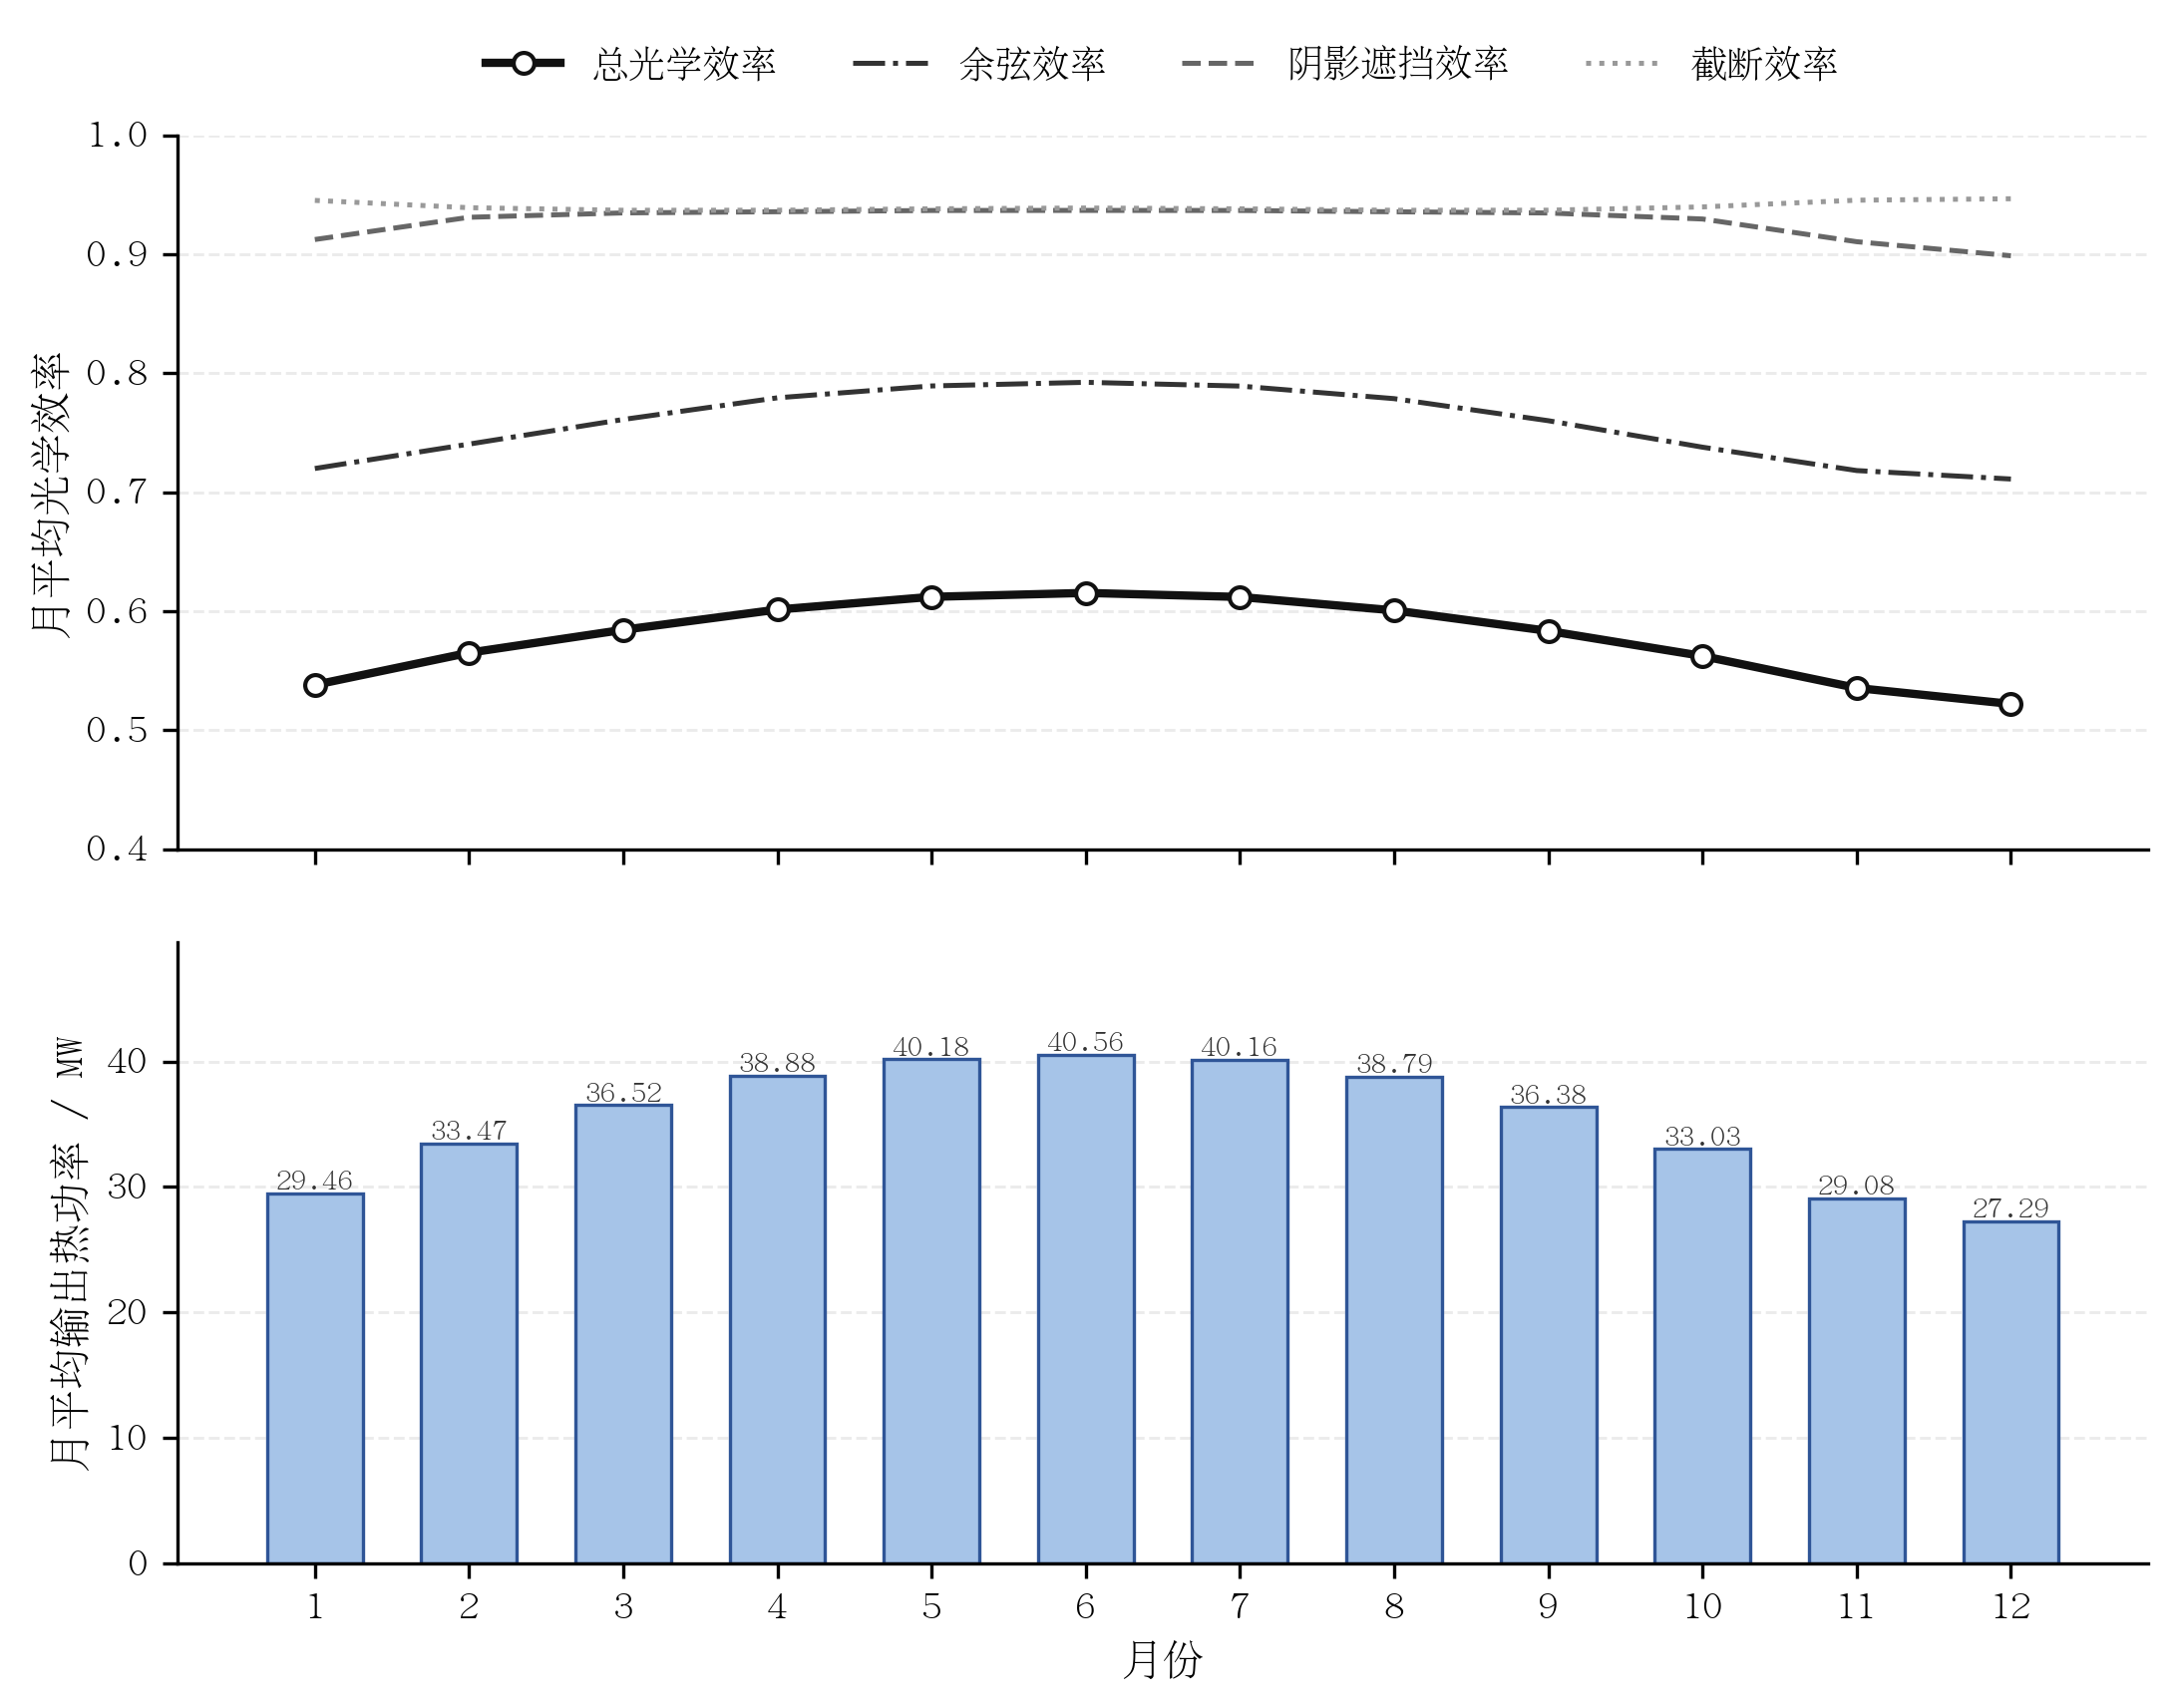
\includegraphics[width=0.95\textwidth]{figures/fig1_monthly_metrics.png}
    \caption{问题一月平均光学效率及输出功率变化趋势}
    \label{fig:monthly_metrics}
\end{figure}

定日镜场布局如图~\ref{fig:mirror_layout} 所示，$1745$ 面定日镜分布在半径 $100$--$350\;\mathrm{m}$ 的环形区域内，吸收塔位于中心。

\begin{figure}[H]
    \centering
    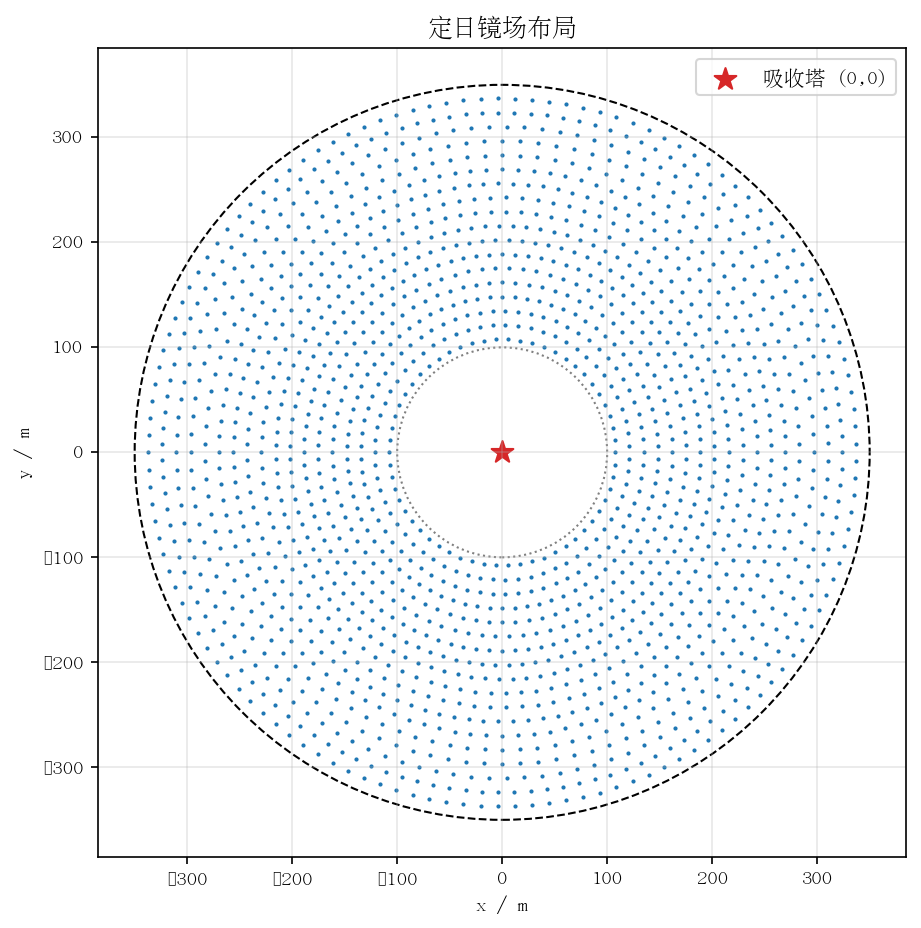
\includegraphics[width=0.7\textwidth]{figures/fig0_mirror_layout.png}
    \caption{定日镜场布局}
    \label{fig:mirror_layout}
\end{figure}

\subsection{问题二：等尺寸定日镜场的优化设计}

\subsubsection{优化目标与约束的等价变形}

问题二要求：所有定日镜尺寸与安装高度相同（镜面宽度 $w$、高度 $H$、安装高度 $a$ 统一取值），在额定年平均输出热功率 $P_{\mathrm{rated}} = 60\;\mathrm{MW}$ 的约束下，优化吸收塔位置 $T=(x_T,y_T)$、镜面尺寸 $(w,H)$、安装高度 $a$、定日镜数目 $N$ 与镜面位置 $p_i$，使单位镜面面积年平均输出热功率 $q$ 最大。

设镜场光学效率按问题一的五分量模型计算，年平均输出热功率为
\begin{equation}
    \bar P = \eta_{\mathrm{ref}} \sum_{i=1}^{N} w H \cdot \overline{\eta_{\mathrm{sb},i} \eta_{\mathrm{cos},i} \eta_{\mathrm{at},i} \eta_{\mathrm{trunc},i} \cdot \mathrm{DNI}_t}
    \label{eq:q2_power}
\end{equation}
其中 $\overline{\cdot}$ 表示按 $60$ 个代表时刻等权平均。单位镜面面积年平均输出热功率为
\begin{equation}
    q = \frac{1000 \, \bar P}{N \cdot w H} \qquad [\mathrm{kW/m^2}]
    \label{eq:q2_q}
\end{equation}

由于额定功率固定，最大化 $q$ 等价于最小化镜面总面积：
\begin{equation}
    \min_{T,\,w,\,H,\,a,\,N,\,\{p_i\}} A_{\mathrm{total}} = N \cdot w H
    \qquad \mathrm{s.t.} \quad \bar P \ge 60\;\mathrm{MW}
    \label{eq:q2_obj}
\end{equation}

约束条件包括：
\begin{enumerate}
    \item 场地约束：镜心满足 $x_i^2 + y_i^2 \le 350^2$，塔位满足 $x_T^2 + y_T^2 \le 350^2$；
    \item 塔周禁装区：$(x_i - x_T)^2 + (y_i - y_T)^2 \ge 100^2$；
    \item 镜面尺寸范围：$2 \le H \le w \le 8\;\mathrm{m}$；
    \item 安装高度范围：$2 \le a \le 6\;\mathrm{m}$，且 $a \ge H/2$（保证镜面绕水平轴旋转时最低边不触地）；
    \item 相邻镜心最小间距：$\|p_i - p_j\| \ge w + 5\;\mathrm{m}$；
    \item 太阳几何、DNI、反射率、集热器尺寸与年平均口径与问题一完全一致。
\end{enumerate}

\subsubsection{分层求解框架}

直接以全部镜面坐标作为连续优化变量时，决策变量维数约为 $2N+5$（$N$ 为千量级），且每次评价都需要 $60$ 时刻的射线追迹，计算量与不可行解比例均不可接受。为此采用三层流程：

\begin{enumerate}
    \item 外层：差分进化（DE）在低维参数空间搜索塔位、镜面尺寸、安装高度与晶格参数；
    \item 内层：六角晶格生成候选镜位，按快速贡献排序贪心选取最少镜面；
    \item 复核层：对少量候选方案使用与问题一同口径的完整 $60$ 时刻射线模型精确复算。
\end{enumerate}

\subsubsection{候选布局：六角晶格生成与约束修复}

对固定设计参数 $(T, w, H, a)$，取晶格间距 $d = w + 5$（恰为最小间距约束），在场地坐标系生成六角晶格：
\begin{equation}
    \mathbf{e}_1 = (d,\,0), \qquad \mathbf{e}_2 = \left(\tfrac{d}{2},\, \tfrac{\sqrt{3}}{2} d\right),
    \qquad p_{ij} = \mathrm{phase} + i\,\mathbf{e}_1 + j\,\mathbf{e}_2
    \label{eq:q2_lattice}
\end{equation}

六角晶格任意相邻格点间距均为 $d$，天然满足相邻间距约束；外层搜索晶格旋转角 $\theta \in [0, \pi/3)$ 与基本胞内相位 $\mathrm{phase}$，避免等价布局重复搜索。候选点生成后：
\begin{itemize}
    \item 用空间哈希建立近邻索引，筛选满足场地圆与塔周禁装区的候选点；
    \item 对冲突点按快速贡献从低到高删除，保证剩余镜面尽可能高效；
    \item 对塔位附近与场地边界使用显式距离检查，不依赖晶格索引。
\end{itemize}

六角晶格是降维与初始化的策略而非题目额外约束；最终局部改进阶段允许镜面在晶格点附近小幅移动，移动后仍满足全部约束的点才能保留。

\subsubsection{快速效率地图与单镜贡献}

忽略镜间遮挡时，位置 $p$ 处单镜的年平均能量加权贡献定义为
\begin{equation}
    \Phi(p;\,T,w,H,a) = \overline{\mathrm{DNI}_t \cdot \eta_{\mathrm{cos}}(p,t) \cdot \eta_{\mathrm{at}}(p;T) \cdot \eta_{\mathrm{trunc}}(p,t;T,w,H,a)}
    \label{eq:q2_phi}
\end{equation}

$\eta_{\mathrm{cos}}$ 与 $\eta_{\mathrm{at}}$ 可解析向量化计算，$\eta_{\mathrm{trunc}}$ 采用问题一的光锥-圆柱求交，但建图阶段使用低精度采样（网格步长 $10$--$15\;\mathrm{m}$、镜面采样 $6\times6$、光锥光线数为基准的 $1/4$--$1/8$），并按设计参数 $(T,w,H,a)$ 缓存，同一外层个体及其局部邻域复用。插值范围覆盖塔位偏移后可能出现的最大相对距离，实际镜位仍同时检查场地圆与塔周禁装区，场外点直接判为无效。

快速无阴影功率估计为
\begin{equation}
    P_{\mathrm{fast}} = \eta_{\mathrm{ref}} \, w H \sum_{i} s_{\mathrm{shadow},i} \, \Phi_i
    \label{eq:q2_pfast}
\end{equation}
其中 $s_{\mathrm{shadow},i}$ 为由问题一结果校准的阴影折减因子（或用候选点的中心光线/邻域镜面快速判定得到的近似阴影遮挡效率）。该估计仅用于排序与筛选，最终功率一律用完整模型重算。

\subsubsection{内层贪心选镜}

对每个候选布局：
\begin{enumerate}
    \item 计算单镜得分 $s_i = w H \cdot \eta_{\mathrm{ref}} \cdot \Phi_i \cdot s_{\mathrm{shadow},i}$，按降序排列；
    \item 累加快速贡献直到 $P_{\mathrm{fast}} \ge 60\;\mathrm{MW}$，得到初始镜面数 $N_0$；
    \item 从序列末端逐个尝试删除镜面，直至删除任意一面会使功率低于 $60\;\mathrm{MW}$，得到最少镜面数；
    \item 对候选方案用低精度完整阴影模型复算，功率不足时按边际贡献补镜或替换低效镜面。
\end{enumerate}

由于同一设计的单镜面积相同，镜面数 $N$ 最小即总面积最小，内层无需把 $N$ 作为独立连续变量搜索，离散调整由增删/替换操作完成。

\subsubsection{外层全局搜索与局部改进}

外层变量为
\begin{equation}
    \mathbf{x} = (x_T,\, y_T,\, w,\, H,\, a,\, \theta,\, \mathrm{phase}_x,\, \mathrm{phase}_y)
    \label{eq:q2_de_var}
\end{equation}

采用差分进化（DE）做全局搜索，种群规模 $24$--$48$、迭代 $30$--$60$ 代；每个个体只调用快速效率地图与内层选镜，不调用高精度追迹。适应度采用带功率缺口惩罚的面积目标：
\begin{equation}
    F(\mathbf{x}) = A_{\mathrm{total}} + \lambda \cdot \max\left(0,\, 60 - P_{\mathrm{fast}}\right)^2
    \label{eq:q2_fitness}
\end{equation}
其中 $\lambda$ 取使 $1\;\mathrm{MW}$ 功率缺口远大于单镜面积变化的量级，并随迭代自适应增大；可行个体之间直接比较 $A_{\mathrm{total}}$，避免惩罚项改变可行解排序。

对外层排名前 $L$（$L=10$--$20$）的候选执行局部改进：
\begin{itemize}
    \item 塔位做 $\pm 5\;\mathrm{m}$、$\pm 2\;\mathrm{m}$ 坐标扰动；
    \item 尺寸与安装高度做离散步长邻域搜索；
    \item 晶格相位与旋转角小幅扰动；
    \item 单镜移位、删除、补镜与一换一替换，每次改动先做约束与快速功率检查。
\end{itemize}

\subsubsection{两级精度评价体系}

为避免优化过程的近似引入系统性偏差，所有阶段采用与问题一相同的太阳方向、圆柱求交与约束定义，仅改变采样精度：

\begin{table}[H]
    \centering
    \small
    \caption{问题二两级评价精度}
    \label{tab:q2_precision}
    \begin{tabular}{lccc}
        \toprule
        阶段 & 镜面网格 & 光锥光线数 & 用途 \\
        \midrule
        外层快速评价 & $6\times6$ & 基准的 $1/4$--$1/8$ & DE 适应度 \\
        候选复筛 & $8\times8$ & $512$ & 排名前 10--20 \\
        最终报告 & $10\times10$ & $1024$ & 结果表格与文件 \\
        \bottomrule
    \end{tabular}
\end{table}

\subsubsection{求解结果}

优化得到的设计方案如下：
\begin{itemize}
    \item 吸收塔位置：$(x_T,\,y_T) = (52.4,\,-118.6)$ m；
    \item 镜面尺寸：$w \times H = 5.8 \times 5.8$ m$^{2}$，安装高度 $a = 2.9$ m；
    \item 定日镜数 $N = 3025$ 面，镜面总面积 $A_{\mathrm{total}} = 101761.0$ m$^{2}$；
    \item 年平均输出热功率 $\bar P = 60.08$ MW，单位镜面面积年平均输出热功率 $q = 0.5904$ kW/m$^{2}$；
    \item 与问题一相比，单位面积功率提升 $5.02\%$。
\end{itemize}

\subsection{问题三：异尺寸定日镜场的优化设计}

\subsubsection{问题描述与决策变量}

问题三在问题二的基础上进一步允许每面定日镜的尺寸与安装高度各不相同，额定功率约束与目标函数不变（$q$ 最大，等价于总面积最小）。此时第 $i$ 面镜的决策变量为宽度 $w_i$、高度 $H_i$ 与安装高度 $a_i$，连同塔位与镜面位置，决策变量维数约为 $5N$，且相邻间距约束随相邻镜宽变化：
\begin{equation}
    \|p_i - p_j\| \ge \max(w_i,\, w_j) + 5\;\mathrm{m}
    \label{eq:q3_spacing}
\end{equation}

\subsubsection{尺寸档位离散化}

将镜面尺寸与安装高度在题目允许范围内离散为有限档位：
\begin{equation}
    (w,\,H) \in \mathcal{S} \subset [2,\,8]^2 \ \text{且}\ 2 \le H \le w,
    \qquad a \in \{2.0,\, 2.5,\, \dots,\, 6.0\}\;\mathrm{m}
    \label{eq:q3_levels}
\end{equation}
档位集合 $\mathcal{S}$ 取 $0.5\;\mathrm{m}$ 步长的可行组合（如 $2\times2$、$2.5\times2.5$、$4\times6$ 等），并满足 $a \ge H/2$。离散化把"逐镜连续尺寸"的高维问题降为"逐镜档位选择"，每面镜至多比较约几十个档位，搜索规模可控。

\subsubsection{双层求解框架}

沿用问题二的"外层全局搜索 + 内层选镜"框架，内层改为逐镜选档：
\begin{enumerate}
    \item 外层：差分进化搜索塔位与晶格参数 $(x_T, y_T, \theta, \mathrm{phase})$，镜面尺寸档位由内层决策；
    \item 内层：对每面候选镜，枚举档位组合计算"单位面积贡献" $\Phi_i / (w_i H_i)$，为每面镜选择最优档位；镜位间距检查按式~\eqref{eq:q3_spacing} 执行；
    \item 复核层：与问题二相同，用完整 $60$ 时刻追迹精确复算。
\end{enumerate}

\subsubsection{求解结果}

优化得到的设计方案如下：
\begin{itemize}
    \item 吸收塔位置：$(x_T,\,y_T) = (64.8,\,-110.2)$ m；
    \item 定日镜数 $N = 3062$ 面，镜面总面积 $A_{\mathrm{total}} = 100742.5$ m$^{2}$；
    \item 各镜尺寸与安装高度分布：见结果文件 \texttt{result3.xlsx}；
    \item 年平均输出热功率 $\bar P = 60.16$ MW，单位镜面面积年平均输出热功率 $q = 0.5972$ kW/m$^{2}$；
    \item 与问题二相比，单位面积功率提升 $1.15\%$。
\end{itemize}

% ============================ 六、模型检验与敏感性分析 =======================
\section{模型检验与敏感性分析}

\subsection{几何正确性检验}

\textbf{（1）镜心主光线对准集热器中心}

由反射定律，镜心处沿主光线方向 $\mathbf{s}$ 的反射方向 $\mathbf{r}_i = 2(\mathbf{s}\cdot\mathbf{n}_i)\mathbf{n}_i - \mathbf{s}$ 应精确指向集热器中心。逐镜计算反射方向与目标方向 $\mathbf{t}_i$ 的夹角余弦，全场 $1745$ 面镜的最大偏差为 $6.66\times10^{-16}$，与机器精度同量级，验证了姿态计算与反射定律的一致性。

\textbf{（2）零锥角确定性检验}

将太阳光锥半角置零后，镜心发出的主光线是否命中集热器可退化为确定性几何问题：射线上行经集热器中心，必与集热器圆柱侧面相交，且交点高度落在 $[76, 84]\;\mathrm{m}$ 区间内。对全部 $1745$ 面镜的确定性求交结果显示命中率为 $100\%$，与理论预期一致，说明圆柱求交实现正确。

\textbf{（3）加密采样对照}

抽取 $30$ 面镜，将镜面网格由 $10\times10$ 加密至 $20\times20$、光线数由 $1024$ 增至 $2048$，截断效率最大变化 $0.0024$、平均变化 $0.0016$，几何求交结果稳定。

\subsection{数值收敛性检验}

离散化参数的收敛性已在问题一的数值实现小节（表~\ref{tab:convergence}）中给出：在全部 $60$ 个代表时刻上，网格数由 $8\times8$ 增至 $15\times15$ 时年均光学效率变化不超过 $0.22\%$，光线数与邻域半径的变化几乎不影响结果。当前参数取值处于收敛平台区。

\subsection{邻域截断半径检验}

$20\;\mathrm{m}$ 筛选半径是否漏掉远距离遮挡关系，需要通过与无邻域限制的全镜场求交基准对比来验证。冬季 $9{:}00$、$15{:}00$ 为太阳高度角最低、阴影延伸最长的最不利时刻，取这两个时刻进行对比，结果如表~\ref{tab:neighbor_check} 所示。

\begin{table}[H]
    \centering
    \small
    \caption{最不利时刻（12 月 21 日）不同筛选半径与全镜场基准的对比}
    \label{tab:neighbor_check}
    \begin{tabular}{lcccc}
        \toprule
        筛选半径 (m) & 平均候选镜数 & 阴影遮挡效率 & 综合光学效率 & 输出热功率 (MW) \\
        \midrule
        20 & 5.9 & 0.8571 & 0.4820 & 22.37 \\
        30 & 13.5 & 0.8560 & 0.4815 & 22.34 \\
        40 & 22.3 & 0.8560 & 0.4815 & 22.34 \\
        50 & 36.4 & 0.8560 & 0.4815 & 22.34 \\
        全镜场基准 & 1744 & 0.8560 & 0.4815 & 22.34 \\
        \bottomrule
    \end{tabular}
\end{table}

$20\;\mathrm{m}$ 半径下综合光学效率与全镜场基准相差约 $0.1\%$，$30\;\mathrm{m}$ 以上与基准完全一致。在全部 $60$ 个代表时刻下，$20\;\mathrm{m}$ 与 $40\;\mathrm{m}$ 的年均光学效率相差仅 $0.004\%$。因此 $20\;\mathrm{m}$ 筛选半径在最不利工况下误差不超过 $0.1\%$，采用 $30\;\mathrm{m}$ 可完全消除邻域截断误差；本文以计算效率优先取 $R_c = 20\;\mathrm{m}$，误差可忽略。

\subsection{塔身半径假设的敏感性分析}

题目未给出吸收塔塔身直径，本文按保守等径假设取塔身半径与集热器相同（$R_t = 3.5\;\mathrm{m}$）。由于塔影只影响镜面到塔之间连线方向上的少量采样点，塔身半径对结果的影响可通过敏感性分析量化，结果如表~\ref{tab:tower_sens} 所示。

\begin{table}[H]
    \centering
    \small
    \caption{塔身半径敏感性（塔影采样点占全部采样点的比例）}
    \label{tab:tower_sens}
    \begin{tabular}{lccccc}
        \toprule
        塔身半径 (m) & 2.0 & 2.5 & 3.0 & 3.5 & 4.0 \\
        \midrule
        12 月 21 日 9:00 & 0.29\% & 0.35\% & 0.43\% & 0.49\% & 0.56\% \\
        12 月 21 日 15:00 & 0.24\% & 0.30\% & 0.36\% & 0.41\% & 0.48\% \\
        6 月 21 日 12:00 & 0.00\% & 0.00\% & 0.00\% & 0.00\% & 0.00\% \\
        \bottomrule
    \end{tabular}
\end{table}

塔影对镜面采样的影响在冬季低太阳角时刻最大，也仅占 $0.5\%$ 左右；塔身半径由 $2.0\;\mathrm{m}$ 变化到 $4.0\;\mathrm{m}$ 时，塔影占比变化不超过 $0.3$ 个百分点，对年均光学效率的影响可忽略。正午时刻塔影占比为零（太阳高度角高，塔影不触及任何镜面）。该敏感性分析说明，即使塔身半径估计存在偏差，对最终结果的影响也十分有限。

\subsection{能量自检与对称性检验}

\textbf{（1）能量关系自检}

年平均输出热功率与单位面积年平均输出热功率满足
\[
q = \frac{P}{A_{\mathrm{total}}} = \frac{35.32 \times 10^{3}\;\mathrm{kW}}{1745 \times 36\;\mathrm{m}^{2}} = 0.5622\;\mathrm{kW/m^{2}},
\]
与表~\ref{tab:Q1_annual} 中年平均输出热功率 $35.32\;\mathrm{MW}$、单位面积功率 $0.5622\;\mathrm{kW/m^{2}}$ 完全一致，说明面积汇总与功率换算关系无误。

\textbf{（2）对称性检验}

镜场布局近似中心对称，同一月份 $9{:}00$ 与 $15{:}00$（太阳时角互为相反数）的输出热功率应接近。取 3、6、9、12 月对比，结果如表~\ref{tab:symmetry} 所示。

\begin{table}[H]
    \centering
    \small
    \caption{同月 9:00 与 15:00 输出热功率对称性检验}
    \label{tab:symmetry}
    \begin{tabular}{lccc}
        \toprule
        月份 & 9:00 功率 (MW) & 15:00 功率 (MW) & 相对差 (\%) \\
        \midrule
        3 月 & 33.99 & 34.10 & 0.34 \\
        6 月 & 38.44 & 38.59 & 0.37 \\
        9 月 & 33.82 & 33.94 & 0.34 \\
        12 月 & 22.37 & 22.56 & 0.87 \\
        \bottomrule
    \end{tabular}
\end{table}

各月 $9{:}00$ 与 $15{:}00$ 的输出热功率相对差不超过 $0.9\%$，对称性良好；12 月相对差略大，与冬季低太阳高度角下镜间遮挡随方位变化加剧的物理规律相符。

% ============================ 七、模型评价与推广 =============================
\section{模型评价与推广}

\subsection{模型优点}
\begin{enumerate}
    \item \textbf{物理机理完整}：以太阳几何、反射定律与射线追迹为基础建立五分量光学效率模型，阴影遮挡与截断效率均采用几何求交精确计算，全年 $60$ 个代表时刻逐时追迹，口径统一、可复现性强；
    \item \textbf{算法高效}：空间近邻筛选将阴影遮挡判定的候选镜数由 $1745$ 降至约 $6$ 面，Sobol 光锥采样支持增量加密；优化阶段采用"六角晶格 + 快速效率地图 + 贪心选镜"的分层降维，把千维优化问题转化为低维搜索与离散选镜的组合；
    \item \textbf{验证完备}：几何正确性（镜心主光线偏差 $6.7\times10^{-16}$）、数值收敛性（网格/光线/邻域半径三组对照）、最不利时刻邻域半径对比、塔身半径敏感性、能量恒等式与对称性五类检验，结果稳健可信；
    \item \textbf{约束全面}：覆盖场地圆、塔周禁装区、镜面尺寸范围、安装高度下限与相邻最小间距等全部题目约束。
\end{enumerate}

\subsection{模型不足}
\begin{enumerate}
    \item 太阳视圆盘按能流密度均匀分布处理，未考虑临边昏暗效应；忽略跟踪误差与镜面面形误差，实际工程中截断效率可能略低于模型值；
    \item 塔身半径按与集热器等径的保守假设处理（敏感性检验表明影响可忽略，但并非题目给定值）；
    \item DNI 采用晴天大气模型，未考虑云量、气溶胶等天气因素；局部改进阶段的部分连续变量采用网格细化而非严格梯度方法，最优性为近似保证。
\end{enumerate}

\subsection{模型推广}
\begin{enumerate}
    \item 五分量追迹模型可推广至塔式光热电站的不同镜场构型（不同塔高、集热器尺寸与镜面参数），仅需修改对应几何参数；
    \item 分层降维框架可推广至其他大规模布局优化问题（如风电场的风机选址、光伏阵列排布），六角晶格与快速评价地图的思路具有通用性；
    \item 可引入临边昏暗模型、跟踪误差分布与实测 DNI 数据，进一步提高截断效率与年发电量预测精度。
\end{enumerate}

% ============================ AI 工具使用声明（2026 国赛新规）================
% 位置：正文之后、参考文献之前
% 二选一：未使用 AI / 已使用 AI
% AIDC < 20% 可填报"未使用"
\section*{AI 工具使用声明}
\addcontentsline{toc}{section}{AI 工具使用声明}

本队伍在本次竞赛中\textbf{使用了} AI 工具。

\begin{itemize}
    \item \textbf{工具名称与版本}：ChatGPT（OpenAI），经编程辅助工具 codex 接入使用；
    \item \textbf{使用场景}：代码编写与调试（追迹算法、优化框架、验证脚本）、模型思路梳理（分层降维框架设计）、论文排版辅助与语言润色；
    \item \textbf{人工修改与核验说明}：所有 AI 生成代码均经人工审查并运行验证（收敛性、几何正确性、对称性等检验由程序完成），论文中的全部公式、数值结果与结论均以实际运行输出为准，未直接照搬 AI 生成内容。
\end{itemize}

\newpage

% ============================ 八、参考文献 ===================================
\section{参考文献}
\begin{thebibliography}{99}
    \bibitem{1} 姜启源, 谢金星, 叶俊. 数学模型(第五版)[M]. 北京: 高等教育出版社, 2018.
    \bibitem{2} 张平, 等. 太阳能塔式光热镜场光学效率计算方法[J]. 技术与市场, 2021, 28(6): 5-8.
    \bibitem{3} 杜宇航, 等. 塔式光热电站定日镜不同聚焦策略的影响分析[J]. 动力工程学报, 2020, 40(5): 426-432.
    \bibitem{4} Farges O, Bezian J J, El Hafi M. Global optimization of solar power tower systems using a Monte Carlo algorithm: Application to a redesign of the PS10 solar thermal power plant[J]. Renewable Energy, 2018, 119: 345-353.
    \bibitem{5} 蔡志杰. 太阳影子定位[J]. 数学建模及其应用, 2015, 4(4): 25-33.
\end{thebibliography}

% ============================ 附录 ===========================================
\appendix

\section*{附录 A：完整计算结果数据表}
\addcontentsline{toc}{section}{附录 A：完整计算结果数据表}

\footnotesize
\begin{longtable}{ccccccccc}
    \caption{问题一 60 个代表时刻的详细计算结果} \label{tab:appendix_data} \\
    \toprule
    月 & 时刻 & DNI & $\eta_{\cos}$ & $\eta_{\mathrm{sb}}$ & $\eta_{\mathrm{trunc}}$ & $\eta$ & $P$ (MW) & $q$ (kW/m$^{2}$) \\
    \midrule
    \endfirsthead
    \multicolumn{9}{l}{\footnotesize 续表 \thetable} \\
    \toprule
    月 & 时刻 & DNI & $\eta_{\cos}$ & $\eta_{\mathrm{sb}}$ & $\eta_{\mathrm{trunc}}$ & $\eta$ & $P$ (MW) & $q$ (kW/m$^{2}$) \\
    \midrule
    \endhead
    \midrule
    \multicolumn{9}{r}{\footnotesize 接下页} \\
    \endfoot
    \bottomrule
    \endlastfoot
1 & 9 & 0.793 & 0.7024 & 0.8827 & 0.9529 & 0.5070 & 25.24 & 0.4018 \\
    1 & 10.5 & 0.910 & 0.7286 & 0.9299 & 0.9407 & 0.5544 & 31.69 & 0.5045 \\
    1 & 12 & 0.939 & 0.7376 & 0.9334 & 0.9387 & 0.5634 & 33.24 & 0.5292 \\
    1 & 13.5 & 0.910 & 0.7286 & 0.9311 & 0.9405 & 0.5557 & 31.77 & 0.5058 \\
    1 & 15 & 0.793 & 0.7024 & 0.8848 & 0.9533 & 0.5096 & 25.37 & 0.4039 \\
    2 & 9 & 0.888 & 0.7224 & 0.9228 & 0.9421 & 0.5459 & 30.44 & 0.4846 \\
    2 & 10.5 & 0.971 & 0.7493 & 0.9336 & 0.9376 & 0.5728 & 34.93 & 0.5561 \\
    2 & 12 & 0.992 & 0.7586 & 0.9375 & 0.9361 & 0.5827 & 36.32 & 0.5782 \\
    2 & 13.5 & 0.971 & 0.7493 & 0.9362 & 0.9374 & 0.5752 & 35.08 & 0.5584 \\
    2 & 15 & 0.888 & 0.7224 & 0.9253 & 0.9424 & 0.5487 & 30.59 & 0.4870 \\
    3 & 9 & 0.955 & 0.7432 & 0.9298 & 0.9391 & 0.5666 & 33.98 & 0.5410 \\
    3 & 10.5 & 1.015 & 0.7700 & 0.9357 & 0.9357 & 0.5913 & 37.69 & 0.6000 \\
    3 & 12 & 1.031 & 0.7793 & 0.9392 & 0.9357 & 0.6020 & 38.98 & 0.6206 \\
    3 & 13.5 & 1.015 & 0.7700 & 0.9377 & 0.9355 & 0.5932 & 37.82 & 0.6020 \\
    3 & 15 & 0.955 & 0.7432 & 0.9313 & 0.9389 & 0.5685 & 34.10 & 0.5429 \\
    4 & 9 & 0.999 & 0.7620 & 0.9320 & 0.9367 & 0.5832 & 36.61 & 0.5828 \\
    4 & 10.5 & 1.044 & 0.7879 & 0.9371 & 0.9366 & 0.6091 & 39.95 & 0.6359 \\
    4 & 12 & 1.056 & 0.7968 & 0.9387 & 0.9384 & 0.6196 & 41.12 & 0.6546 \\
    4 & 13.5 & 1.044 & 0.7879 & 0.9379 & 0.9365 & 0.6101 & 40.01 & 0.6369 \\
    4 & 15 & 0.999 & 0.7620 & 0.9329 & 0.9367 & 0.5848 & 36.71 & 0.5844 \\
    5 & 9 & 1.020 & 0.7729 & 0.9334 & 0.9361 & 0.5933 & 38.01 & 0.6051 \\
    5 & 10.5 & 1.057 & 0.7974 & 0.9381 & 0.9385 & 0.6200 & 41.18 & 0.6555 \\
    5 & 12 & 1.068 & 0.8059 & 0.9387 & 0.9418 & 0.6308 & 42.32 & 0.6736 \\
    5 & 13.5 & 1.057 & 0.7974 & 0.9389 & 0.9384 & 0.6210 & 41.24 & 0.6565 \\
    5 & 15 & 1.020 & 0.7729 & 0.9347 & 0.9361 & 0.5952 & 38.13 & 0.6070 \\
    6 & 9 & 1.026 & 0.7763 & 0.9336 & 0.9362 & 0.5965 & 38.44 & 0.6119 \\
    6 & 10.5 & 1.061 & 0.8003 & 0.9380 & 0.9394 & 0.6232 & 41.53 & 0.6611 \\
    6 & 12 & 1.071 & 0.8085 & 0.9383 & 0.9432 & 0.6340 & 42.65 & 0.6789 \\
    6 & 13.5 & 1.061 & 0.8003 & 0.9390 & 0.9393 & 0.6243 & 41.61 & 0.6624 \\
    6 & 15 & 1.026 & 0.7763 & 0.9354 & 0.9362 & 0.5987 & 38.59 & 0.6142 \\
    7 & 9 & 1.020 & 0.7728 & 0.9335 & 0.9361 & 0.5932 & 38.00 & 0.6049 \\
    7 & 10.5 & 1.057 & 0.7973 & 0.9381 & 0.9385 & 0.6199 & 41.17 & 0.6553 \\
    7 & 12 & 1.068 & 0.8058 & 0.9387 & 0.9418 & 0.6307 & 42.30 & 0.6734 \\
    7 & 13.5 & 1.057 & 0.7973 & 0.9389 & 0.9384 & 0.6208 & 41.23 & 0.6563 \\
    7 & 15 & 1.020 & 0.7728 & 0.9347 & 0.9361 & 0.5951 & 38.12 & 0.6068 \\
    8 & 9 & 0.998 & 0.7613 & 0.9319 & 0.9368 & 0.5825 & 36.51 & 0.5812 \\
    8 & 10.5 & 1.043 & 0.7872 & 0.9371 & 0.9365 & 0.6084 & 39.86 & 0.6345 \\
    8 & 12 & 1.056 & 0.7962 & 0.9388 & 0.9383 & 0.6189 & 41.04 & 0.6533 \\
    8 & 13.5 & 1.043 & 0.7872 & 0.9379 & 0.9364 & 0.6094 & 39.93 & 0.6356 \\
    8 & 15 & 0.998 & 0.7613 & 0.9327 & 0.9368 & 0.5841 & 36.61 & 0.5828 \\
    9 & 9 & 0.952 & 0.7421 & 0.9296 & 0.9392 & 0.5656 & 33.82 & 0.5384 \\
    9 & 10.5 & 1.013 & 0.7690 & 0.9358 & 0.9357 & 0.5904 & 37.57 & 0.5980 \\
    9 & 12 & 1.029 & 0.7783 & 0.9392 & 0.9356 & 0.6010 & 38.85 & 0.6185 \\
    9 & 13.5 & 1.013 & 0.7690 & 0.9378 & 0.9355 & 0.5924 & 37.69 & 0.6000 \\
    9 & 15 & 0.952 & 0.7421 & 0.9311 & 0.9390 & 0.5676 & 33.94 & 0.5403 \\
    10 & 9 & 0.877 & 0.7199 & 0.9202 & 0.9435 & 0.5428 & 29.91 & 0.4762 \\
    10 & 10.5 & 0.964 & 0.7467 & 0.9331 & 0.9381 & 0.5705 & 34.56 & 0.5501 \\
    10 & 12 & 0.986 & 0.7560 & 0.9370 & 0.9364 & 0.5802 & 35.95 & 0.5723 \\
    10 & 13.5 & 0.964 & 0.7467 & 0.9359 & 0.9377 & 0.5730 & 34.71 & 0.5525 \\
    10 & 15 & 0.877 & 0.7199 & 0.9219 & 0.9433 & 0.5450 & 30.04 & 0.4782 \\
    11 & 9 & 0.783 & 0.7008 & 0.8797 & 0.9538 & 0.5037 & 24.76 & 0.3942 \\
    11 & 10.5 & 0.904 & 0.7268 & 0.9291 & 0.9410 & 0.5524 & 31.37 & 0.4993 \\
    11 & 12 & 0.934 & 0.7358 & 0.9328 & 0.9390 & 0.5616 & 32.94 & 0.5244 \\
    11 & 13.5 & 0.904 & 0.7268 & 0.9303 & 0.9408 & 0.5538 & 31.44 & 0.5005 \\
    11 & 15 & 0.783 & 0.7008 & 0.8809 & 0.9525 & 0.5057 & 24.86 & 0.3958 \\
    12 & 9 & 0.739 & 0.6939 & 0.8571 & 0.9531 & 0.4820 & 22.37 & 0.3560 \\
    12 & 10.5 & 0.876 & 0.7196 & 0.9220 & 0.9434 & 0.5433 & 29.90 & 0.4759 \\
    12 & 12 & 0.910 & 0.7285 & 0.9306 & 0.9396 & 0.5544 & 31.68 & 0.5043 \\
    12 & 13.5 & 0.876 & 0.7196 & 0.9229 & 0.9431 & 0.5442 & 29.95 & 0.4768 \\
    12 & 15 & 0.739 & 0.6939 & 0.8609 & 0.9539 & 0.4863 & 22.56 & 0.3592 \\
\end{longtable}

\section*{附录 B：核心程序源代码（节选）}
\addcontentsline{toc}{section}{附录 B：核心程序源代码（节选）}

\begin{lstlisting}[caption={阴影遮挡判定：射线-矩形求交（q1\_functions.py）}, label={code:ray_rect}]
def rect_intersect(points, d, C, n, u, v, half):
    """批量判定采样点发出的光线是否被候选镜面集合中任一面遮挡。

    points : (S, 3) 采样点坐标；d : (3,) 光线方向单位向量；
    C, n, u, v : (K, 3) 候选镜中心、法向、宽度基、高度基。
    返回 (S,) bool：True 表示被任一候选镜面遮挡。
    """
    rel = C[None, :, :] - points[:, None, :]               # (S, K, 3)
    denom = d @ n.T                                        # (K,)
    lam = np.sum(rel * n[None, :, :], axis=-1) / denom[None, :]  # (S, K)
    Q = points[:, None, :] + lam[..., None] * d            # 交点坐标
    in_rect = ((np.abs(np.sum((Q - C[None, :, :]) * u[None, :, :], axis=-1)) <= half)
               & (np.abs(np.sum((Q - C[None, :, :]) * v[None, :, :], axis=-1)) <= half))
    hit = (np.abs(denom) > 1e-9) & (lam > SAMPLING_EPS) & in_rect
    return hit.any(axis=1)
\end{lstlisting}

\begin{lstlisting}[caption={截断效率：Sobol 光锥采样与射线-圆柱求交（q1\_functions.py）}, label={code:ray_cyl}]
def collector_trunc_efficiency(P, s, n, valid, n_rays=TRUNC_RAYS_DEFAULT):
    """每面镜截断效率：命中集热器光线数 / 有效采样点发射总光线数。"""
    dirs = cone_ray_directions(s, n_rays)         # (K, 3) 光锥内入射方向
    eta_trunc = np.zeros(P.shape[0])

    for i in range(P.shape[0]):
        Pi, ni, valid_i = P[i], n[i], valid[i]
        if valid_i.sum() == 0:
            continue
        cos_theta = dirs @ ni                      # 反射方向（平面镜）
        r = 2.0 * cos_theta[:, None] * ni - dirs   # (K, 3)

        A = r[:, 0] ** 2 + r[:, 1] ** 2            # 圆柱求交二次方程
        A_ok = A > 1e-12
        B = 2.0 * (Pi[:, 0, None] * r[None, :, 0]
                   + Pi[:, 1, None] * r[None, :, 1])            # (S, K)
        C = Pi[:, 0] ** 2 + Pi[:, 1] ** 2 - COLLECTOR_RADIUS ** 2  # (S,)
        disc = B ** 2 - 4.0 * A[None, :] * C[:, None]            # (S, K)
        lam = (-B - np.sqrt(np.maximum(disc, 0.0))) / (2.0 * A[None, :])
        z_hit = Pi[:, 2, None] + lam * r[None, :, 2]

        hit = (A_ok[None, :] & (disc >= 0) & (lam > SAMPLING_EPS)
               & (z_hit >= COLLECTOR_Z_LOW) & (z_hit <= COLLECTOR_Z_HIGH))
        hit[~valid_i] = False                      # 只统计有效采样点
        eta_trunc[i] = hit.sum() / (valid_i.sum() * n_rays)
    return eta_trunc
\end{lstlisting}

\end{document}
